\chapter{Cornerstone models: Conjugate families}\label{chap4}

We will introduce conjugate families in basic statistical models with examples, solving them analytically and computationally using R. We will have some mathematical, and computational exercises in R.

\section{Motivation of conjugate families}\label{sec41}

Observing the three fundamental pieces of Bayesian analysis: the posterior distribution (parameter inference), the marginal likelihood (hypothesis testing), and the predictive distribution (prediction), equations \ref{eq:411}, \ref{eq:412} and \ref{eq:413}, respectively, 

\begin{align}
	\pi(\bm{\theta}|\mathbf{y})&=\frac{p(\mathbf{y}|\bm{\theta}) \times \pi(\bm{\theta})}{p(\mathbf{y})},
	\label{eq:411}
\end{align}

\begin{equation}
	p(\mathbf{y})=\int_{\mathbf{\Theta}}p(\mathbf{y}|\bm{\theta})\pi(\bm{\theta})d\bm{\theta},
	\label{eq:412}
\end{equation}

and 

\begin{equation}
	p(\mathbf{Y}_0|\mathbf{y})=\int_{\mathbf{\Theta}}p(\mathbf{Y}_0|\bm{\theta})\pi(\bm{\theta}|\mathbf{y})d\bm{\theta},
	\label{eq:413}
\end{equation}

we can understand that some of the initial limitations of the application of the Bayesian analysis were associated with the absence of algorithms to draw from non-standard posterior distributions (equation \ref{eq:411}), and the lack of analytical solutions of the marginal likelihood (equation \ref{eq:412}) and the predictive distribution (equation \ref{eq:413}). Both issues requiring computational power.

Although there were algorithms to sample from non-standard posterior distributions since the second half of the last century \cite{metropolis53,hastings70,Geman1984}, their particular application in the Bayesian framework emerged later \cite{Gelfand1990,tierney1994markov}, maybe until the increasing computational power of desktop computers. However, it is also common practice nowadays to use models that have standard conditional posterior distributions to mitigate computational requirements. In addition, nice mathematical tricks plus computational algorithms \cite{gelfand1994bayesian, chib1995marginal, chib2001marginal} and approximations \cite{Tierney1986,Jordan1999} are used to obtain the marginal likelihood (prior predictive).

Despite these advances, there are two potentially conflicting desirable model specification features that we can see from equations \ref{eq:411}, \ref{eq:412} and \ref{eq:413}: (1) analytical solutions and (2) the posterior distribution in the same family as the prior distribution for a given likelihood. The latter is called \textit{conjugate priors}, a family of priors that is closed under sampling \cite{schlaifer1961applied}.

These features are desirable as the former implies facility to perform hypothesis testing and predictive analysis, and the latter means invariance of the prior-to-posterior updating. Both features imply less computational burden.

We can easily achieve each of these features independently, for instance using improper priors for analytical tractability, and defining in a broad sense the family of prior distributions for prior conjugacy. However, these features are in conflict. 

Fortunately, we can achieve these two nice characteristics if we assume that the data generating process is given by a distribution function in the \textit{exponential family}. That is, given a random sample $\mathbf{y}=[y_1,y_2,\dots,y_N]^{\top}$, a probability density function $p(\mathbf{y}|\bm{\theta})$ belongs to the exponential family if it has the form

\begin{align}
	p(\mathbf{y}|\bm{\theta})&=\prod_{i=1}^N h(y_i) C(\bm{\theta}) \exp\left\{\eta(\bm{\theta})^{\top}\mathbf{T}(y_i)\right\}\label{eq:414}\\ 
	&=h(\mathbf{y}) C(\bm{\theta})^N\exp\left\{\eta(\bm{\theta})^{\top}\mathbf{T}(\mathbf{y})\right\}\nonumber \\
	&=h(\mathbf{y})\exp\left\{\eta(\bm{\theta})^{\top}\mathbf{T}(\mathbf{y})-A(\bm{\theta})\right\}\nonumber,
\end{align}

where $h(\mathbf{y})=\prod_{i=1}^N h(y_i)$ is a non-negative function, $\eta(\bm{\theta})$ is a known function of the parameters, $A(\bm{\theta})=\log\left\{\int_{\mathbf{Y}}h(\mathbf{y})\exp\left\{\eta(\bm{\theta})^{\top}\mathbf{T}(\mathbf{y})\right\}d\mathbf{y}\right\}=-N\log(C(\bm{\theta}))$ is a normalization factor, and $\mathbf{T}(\mathbf{y})=\sum_{i=1}^N\mathbf{T}(y_i)$ is the vector of sufficient statistics of the distribution (by the factorization theorem).  

If the support of $\mathbf{y}$ is independent of $\bm{\theta}$, then the family is said to be \textit{regular}, otherwise it is \text{irregular}. In addition, if we set $\eta=\eta(\bm{\theta})$, then the exponential family is said to be in the \textit{canonical form} 

\begin{align}
	p(\mathbf{y}|\bm{\theta})&=h(\mathbf{y})D(\bm{\eta})^N\exp\left\{\eta^{\top}\mathbf{T}(\mathbf{y})\right\}\nonumber\\
	&=h(\mathbf{y})\exp\left\{\eta^{\top}\mathbf{T}(\mathbf{y})-B(\bm{\eta})\right\}.\nonumber
\end{align}

A nice feature of this representation is that $\mathbb{E}[\mathbf{T}(\mathbf{y})|\bm{\eta}]=\nabla B(\bm{\eta})$ and $Var[\mathbf{T}(\mathbf{y})|\bm{\eta}]=\nabla^2 B(\bm{\eta})$. 

\subsection{Examples of exponential family distributions}

\begin{enumerate}

\item \textbf{Discrete distributions}

Let's show that some of the most common distributions for random variables that can take values on a finite or countably infinite set are part of the exponential family.
 
\textbf{Poisson distribution} 

Given a random sample $\mathbf{y}=[y_1,y_2,\dots,y_N]^{\top}$ from a \textit{Poisson distribution} let's show that $p(\mathbf{y}|\lambda)$ is in the exponential family.

\begin{align}
	p(\mathbf{y}|\lambda)&=\prod_{i=1}^N \frac{\lambda^{y_i} \exp(-\lambda)}{y_i!}\nonumber\\
	&=\frac{\lambda^{\sum_{i=1}^N y_i}\exp(-N\lambda)}{\prod_{i=1}^N y_i!}\nonumber\\
	&=\frac{\exp(-N\lambda)\exp(\sum_{i=1}^Ny_i\log(\lambda))}{\prod_{i=1}^N y_i!}\nonumber,
\end{align}

then $h(\mathbf{y})=\left[\prod_{i=1}^N y_i!\right]^{-1}$, $\eta(\lambda)=\log(\lambda)$, $T(\mathbf{y})=\sum_{i=1}^N y_i$ (sufficient statistic) and $C(\lambda)=\exp(-\lambda)$.

If we set $\eta=\log(\lambda)$, then 

\begin{align}
	p(\mathbf{y}|\eta)&=\frac{\exp(\eta\sum_{i=1}^Ny_i-N\exp(\eta))}{\prod_{i=1}^N y_i!},\nonumber
\end{align}

such that $B(\eta)=N\exp(\eta)$, then $\nabla(B(\eta))=N\exp(\eta)=N\lambda=\mathbb{E}\left[\sum_{i=1}^N y_i\biggr\rvert\lambda\right]$, that is, $\mathbb{E}\left[\frac{\sum_{i=1}^N y_i}{N}\biggr\rvert\lambda\right]=\mathbb{E}[\bar{y}|\lambda]=\lambda$, and $\nabla^2(B(\eta))=N\exp(\eta)=N\lambda=Var\left[\sum_{i=1}^N y_i\biggr\rvert\lambda\right]=N^2 \times Var\left[\bar{y}\rvert\lambda\right]$, then $Var\left[\bar{y}\rvert\lambda\right]=\frac{\lambda}{N}$.\\ 

\textbf{Bernoulli distribution}

Given a random sample $\mathbf{y}=[y_1,y_2,\dots,y_N]^{\top}$ from a \textit{Bernoulli distribution} let's show that $p(\mathbf{y}|\theta)$ is in the exponential family.


\begin{align}
	p(\mathbf{y}|\theta)&=\prod_{i=1}^N \theta^{y_i}(1-\theta)^{1-y_i}\nonumber\\
	&=\theta^{\sum_{i=1}^N y_i}(1-\theta)^{N-\sum_{i=1}^N y_i}\nonumber\\
	&=(1-\theta)^N\exp\left\{\sum_{i=1}^N y_i\log\left(\frac{\theta}{1-\theta}\right)\right\}\nonumber,
\end{align}

then $h(\mathbf{y})=\mathbb{I}[y_i\in\left\{0,1\right\}]$ (indicator function), $\eta(\theta)=\log\left(\frac{\theta}{1-\theta}\right)$, $T(\mathbf{y})=\sum_{i=1}^N y_i$ and $C(\theta)=1-\theta$.

Write this distribution in the canonical form, and find the mean and variance of the sufficient statistic (Exercise 1).\\ 

\textbf{Multinomial distribution} 

Given a random sample $\mathbf{y}=[\mathbf{y}_1,\mathbf{y}_2,\dots,\mathbf{y}_N]$ from a \textit{m-dimensional multinomial distribution}, where $\mathbf{y}_i=\left[y_{i1},\dots,y_{im}\right]$, $\sum_{l=1}^m y_{il}=n$, $n$ independent trials each of which leads to a success for exactly one of $m$ categories with probabilities $\bm{\theta}=[\theta_1,\theta_2,\dots,\theta_m]$, $\sum_{l=1}^m \theta_l=1$. Let's show that $p(\mathbf{y}|\bm{\theta})$ is in the exponential family.


\begin{align}
	p(\mathbf{y}|\bm{\theta})&=\prod_{i=1}^N \frac{n!}{\prod_{l=1}^m y_{il}!} \prod_{l=1}^m\theta_l^{y_{il}}\nonumber\\
	&=\frac{(n!)^N}{\prod_{i=1}^N\prod_{l=1}^m y_{il}!}\exp\left\{\sum_{i=1}^N\sum_{l=1}^m y_{il}\log(\theta_l)\right\}\nonumber\\
	&=\frac{(n!)^N}{\prod_{i=1}^N\prod_{l=1}^m y_{il}!}\exp\left\{\left(N\times n-\sum_{i=1}^N\sum_{l=1}^{m-1}y_{il}\right)\log(\theta_m)\nonumber\right. \\
	&\left.+\sum_{i=1}^N\sum_{l=1}^{m-1}y_{il}\log(\theta_l)\right\}\nonumber\\
	&=\frac{(n!)^N}{\prod_{i=1}^N\prod_{l=1}^m y_{il}!}\theta_m^{N\times n}\exp\left\{\sum_{i=1}^N\sum_{l=1}^{m-1}y_{il}\log(\theta_l/\theta_m)\right\}\nonumber,
\end{align}

then $h(\mathbf{y})=\frac{(n!)^N}{\prod_{i=1}^N\prod_{l=1}^m y_{il}!}$, $\eta(\bm{\theta})=\left[\log\left(\frac{\theta_1}{\theta_m}\right)\dots \log\left(\frac{\theta_{m-1}}{\theta_m}\right)\right]$, $T(\mathbf{y})=\left[\sum_{i=1}^N y_{i1}\dots \sum_{i=1}^N y_{im-1}\right]$ and $C(\bm{\theta})=\theta_m^n$.\\

\item \textbf{Continuous distributions}

Let's show that some of the most common distributions for random variables that can take any value within a certain range or interval, often an infinite number of possible values, are part of the exponential family.

\textbf{Normal distribution} 

Given a random sample $\mathbf{y}=[y_1,y_2,\dots,y_N]^{\top}$ from a \textit{normal distribution} let's show that $p(\mathbf{y}|\mu,\sigma^2)$ is in the exponential family.

\begin{align}
	p(\mathbf{y}|\mu,\sigma^2)&=\prod_{i=1}^N \frac{1}{2\pi\sigma^2}\exp\left\{-\frac{1}{2\sigma^2}\left(y_i-\mu\right)^2\right\}\nonumber\\
	&= (2\pi)^{-N/2}(\sigma^2)^{-N/2}\exp\left\{-\frac{1}{2\sigma^2}\sum_{i=1}^N\left(y_i-\mu\right)^2\right\}\nonumber\\
	&= (2\pi)^{-N/2}\exp\left\{-\frac{1}{2\sigma^2}\sum_{i=1}^Ny_i^2+\frac{\mu}{\sigma^2}\sum_{i=1}^N y_i\right.\nonumber\\
	&-\left.N\frac{\mu^2}{2\sigma^2}-\frac{N}{2}\log(\sigma^2)\right\}\nonumber,	
\end{align}

then $h(\mathbf{y})=(2\pi)^{-N/2}$, $\eta(\mu,\sigma^2)=\left[\frac{\mu}{\sigma^2} \ \frac{-1}{2\sigma^2}\right]$, $T(\mathbf{y})=\left[\sum_{i=1}^N y_i \ \sum_{i=1}^N y_i^2\right]$ and $C(\mu,\sigma^2)=\exp\left\{-\frac{\mu^2}{2\sigma^2}-\frac{\log(\sigma^2)}{2}\right\}$.

Observe that 

\begin{align}
	p(\mathbf{y}|\mu,\sigma^2)&= (2\pi)^{-N/2}\exp\left\{\eta_1\sum_{i=1}^N y_i+\eta_2\sum_{i=1}^Ny_i^2-\frac{N}{2}\log(-2\eta_2)+\frac{N}{4}\frac{\eta_1^2}{\eta_2}\right\}\nonumber,
\end{align}

where $B(\bm{\eta})=\frac{N}{2}\log(-2\eta_2)-\frac{N}{4}\frac{\eta_1^2}{\eta_2}$. Then,

\begin{align*}
	\nabla B(\bm{\eta}) & = \begin{bmatrix}
		-\frac{N}{2}\frac{\eta_1}{\eta_2}\\
		-\frac{N}{2}\frac{1}{\eta_2}+\frac{N}{4}\frac{\eta_1^2}{\eta_2^2}
	\end{bmatrix}
	=
	\begin{bmatrix}
		N\times\mu\\
		N\times(\mu^2+\sigma^2)
	\end{bmatrix}  = \begin{bmatrix}
		\mathbb{E}\left[\sum_{i=1}^N y_i\bigr\rvert \mu,\sigma^2\right]\\
		\mathbb{E}\left[\sum_{i=1}^N y_i^2\bigr\rvert \mu,\sigma^2\right]
	\end{bmatrix}. 
\end{align*}
\\

\textbf{Multivariate normal distribution}

Given $\mathbf{Y}=[\mathbf{y}_1 \ \mathbf{y}_2 \ \dots \ \mathbf{y}_p]$ a $N\times p$ matrix such that $\mathbf{y}_i\sim N_p(\bm{\mu},\bm{\Sigma})$, $i=1,2,\dots,N$, that is, each $i$-th row of $\mathbf{Y}$ follows a \textit{multivariate normal distribution}. Then, assuming independence between rows, let's show that $p(\mathbf{y}_1,\mathbf{y}_2,\dots,\mathbf{y}_N|\bm{\mu},\bm{\Sigma})$ is in the exponential family.

{\footnotesize{
\begin{align}
	p(\mathbf{y}_1,\dots,\mathbf{y}_N|\bm{\mu},\bm{\Sigma})&=\prod_{i=1}^N (2\pi)^{-p/2}|\Sigma|^{-1/2}\exp\left\{-\frac{1}{2}\left(\mathbf{y}_i-\bm{\mu}\right)^{\top}\bm{\Sigma}^{-1}\left(\mathbf{y}_i-\bm{\mu}\right)\right\}\nonumber\\
	&= (2\pi)^{-pN/2}|\Sigma|^{-N/2}\exp\left\{-\frac{1}{2}tr\left[\sum_{i=1}^N\left(\mathbf{y}_i-\bm{\mu}\right)^{\top}\bm{\Sigma}^{-1}\left(\mathbf{y}_i-\bm{\mu}\right)\right]\right\}\nonumber\\
	&= (2\pi)^{-p N/2}|\Sigma|^{-N/2}\exp\left\{-\frac{1}{2}tr\left[\left(\mathbf{S}+N\left(\bm{\mu}-\hat{\bm{\mu}}\right)\left(\bm{\mu}-\hat{\bm{\mu}}\right)^{\top}\right)\bm{\Sigma}^{-1}\right]\right\}\nonumber\\
	&= (2\pi)^{-p N/2}\exp\left\{-\frac{1}{2}\left[\left(vec\left(\mathbf{S}\right)^{\top}+N vec\left(\hat{\bm{\mu}}\hat{\bm{\mu}}^{\top}\right)^{\top}\right)vec \left(\bm{\Sigma}^{-1}\right)\right.\right.\nonumber\\
	&\left.\left.-2N\hat{\bm{\mu}}^{\top}vec\left(\bm{\mu}^{\top}\bm{\Sigma}^{-1}\right)+N tr\left(\bm{\mu}\bm{\mu}^{\top}\bm{\Sigma}^{-1}\right)+N\log (|\bm{\Sigma}|)\right]\right\}\nonumber,
\end{align}
}}

where the second line uses the trace operator ($tr$), and its invariability under cyclic permutation is used in the third line. In addition, we add and subtract $\hat{\bm{\mu}}=\frac{1}{N}\sum_{i=1}^N\mathbf{y}_i$ in each parenthesis such that we get $\mathbf{S}=\sum_{i=1}^N\left(\mathbf{y}_i-\hat{\bm{\mu}}\right)\left(\mathbf{y}_i-\hat{\bm{\mu}}\right)^{\top}$. We get the fourth line after collecting terms, and using some properties of the trace operator to introduce the vectorization operator ($vec$), that is, $tr({\bf{AB}})=vec({\bf{A}}^{\top})^{\top}vec({\bf{B}})$, and $vec({\bf{A}}+{\bf{B}})=vec({\bf{A}})+vec({\bf{B}})$.

Then $h(\mathbf{y})=(2\pi)^{-pN/2}$, $\eta(\bm{\mu},\bm{\Sigma})^{\top}=\left[\left(vec\left(\bm{\Sigma}^{-1}\right)\right)^{\top} \ \ \left(vec\left(\bm{\mu}^{\top}\bm{\Sigma}^{-1}\right)\right)^{\top}\right]$, $T(\mathbf{y})=\left[-\frac{1}{2}\left(vec\left(\mathbf{S}\right)^{\top}+N vec\left(\hat{\bm{\mu}}\hat{\bm{\mu}}^{\top}\right)^{\top}\right) \ \ -N\hat{\bm{\mu}}^{\top}\right]^{\top}$ and $C(\bm{\mu},\bm{\Sigma})=\exp\left\{-\frac{1}{2}\left(tr\left(\bm{\mu}\bm{\mu}^{\top}\bm{\Sigma}^{-1}\right)+\log(|\Sigma|)\right)\right\}$.
\end{enumerate}

\section{Conjugate prior to exponential family}\label{sec42}

\textbf{Theorem 4.2.1}

The prior distribution $\pi(\bm{\theta})\propto C(\bm{\theta})^{b_0}\exp\left\{\eta(\bm{\theta})^{\top}\mathbf{a}_0\right\}$ is conjugate to the exponential family (equation \ref{eq:414}).\\

\textbf{Proof}
\begin{align}
	\pi(\bm{\theta}|\mathbf{y})& \propto C(\bm{\theta})^{b_0}\exp\left\{\eta(\bm{\theta})^{\top}\mathbf{a}_0\right\} \times h(\mathbf{y}) C(\bm{\theta})^N\exp\left\{\eta(\bm{\theta})^{\top}\mathbf{T}(\mathbf{y})\right\}\nonumber\\
	& \propto C(\bm{\theta})^{N+b_0} \exp\left\{\eta(\bm{\theta})^{\top}(\mathbf{T}(\mathbf{y})+\mathbf{a}_0)\right\}.\nonumber 
\end{align}

Observe that the posterior is in the exponential family, $\pi(\bm{\theta}|\mathbf{y})\propto C(\bm{\theta})^{\beta_n} \exp\left\{\eta(\bm{\theta})^{\top}\mathbf{\alpha}_n\right\}$, $\beta_n=N+b_0$ and $\mathbf{\alpha}_n=\mathbf{T}(\mathbf{y})+\mathbf{a}_0$.\\

\textbf{Remarks}

We see comparing the prior and the likelihood that $b_0$ plays the role of a hypothetical sample size, and $\mathbf{a}_0$ plays the role of hypothetical sufficient statistics. This view helps the elicitation process.

We established the result in the \textit{standard form} of the exponential family. We can also establish this result in the \textit{canonical form} of the exponential family. Observe that given $\bm{\eta}=\bm{\eta}(\bm{\theta})$, another way to get a prior for $\bm{\eta}$ is to use the change of variable theorem given a bijective function.

In the setting where there is a regular conjugate prior, \cite{diaconis1979conjugate} show that we obtain a posterior expectation of the sufficient statistics that is a weighted average between the prior expectation and the likelihood estimate. 

\subsection{Examples: Theorem 4.2.1}\label{sec421}

\begin{enumerate}
	\item \textbf{Likelihood functions from discrete distributions}

\textbf{The Poisson-gamma model}

Given a random sample $\mathbf{y}=[y_1,y_2,\dots,y_N]^{\top}$ from a Poisson distribution then a conjugate prior density for $\lambda$ has the form 

\begin{align}
	\pi(\lambda)&\propto \left(\exp(-\lambda)\right)^{b_0} \exp\left\{a_0\log(\lambda)\right\}\nonumber\\
	& = \exp(-\lambda b_0) \lambda^{a_0}\nonumber\\
	& = \exp(-\lambda \beta_0) \lambda^{\alpha_0-1}.\nonumber
\end{align}

This is the kernel of a gamma density in the \textit{rate parametrization}, $G(\alpha_0,\beta_0)$, $\alpha_0=a_0+1$ and $\beta_0=b_0$.\footnote{Another parametrization of the gamma density is the \textit{scale parametrization} where $\kappa_0=1/\beta_0$. See the health insurance example in Chapter \ref{chap1}.} Then, a prior conjugate distribution for the Poisson likelihood is a gamma distribution.   

Taking into account that $\sum_{i=1}^N y_i$ is a sufficient statistic for the Poisson distribution, then we can think about $a_0$ as the number of occurrences in $b_0$ experiments. 
Observe that

\begin{align}
	\pi(\lambda|\mathbf{y})&\propto \exp(-\lambda \beta_0) \lambda^{\alpha_0-1} \times \exp(-N\lambda)\lambda^{\sum_{i=1}^Ny_i}\nonumber\\
	&= \exp(-\lambda(N+\beta_0)) \lambda^{\sum_{i=1}^Ny_i+\alpha_0-1}.\nonumber 
\end{align}

As expected, this is the kernel of a gamma distribution, which means $\lambda|\mathbf{y}\sim G(\alpha_n,\beta_n)$, $\alpha_n=\sum_{i=1}^Ny_i+\alpha_0$ and $\beta_n=N+\beta_0$.

Observe that $\alpha_0/\beta_0$ is the prior mean, and $\alpha_0/\beta_0^2$ is the prior variance. Then, $\alpha_0\rightarrow 0$ and $\beta_0\rightarrow 0$ imply a non-informative prior such that the posterior mean converges to the maximum likelihood estimator $\bar{y}=\frac{\sum_{i=1}^N y_i}{N}$,

\begin{align}
	\mathbb{E}\left[\lambda|\mathbf{y}\right]&=\frac{\alpha_n}{\beta_n}\nonumber\\
	&=\frac{\sum_{i=1}^Ny_i+\alpha_0}{N+\beta_0}\nonumber\\
	&=\frac{N\bar{y}}{N+\beta_0}+\frac{\alpha_0}{N+\beta_0}.\nonumber
\end{align}

The posterior mean is a weighted average between sample and prior information. This is a general result from regular conjugate priors \cite{diaconis1979conjugate}. Observe that $\mathbb{E}\left[\lambda|\mathbf{y}\right]=\bar{y}, \lim N\rightarrow\infty$. 

In addition, $\alpha_0\rightarrow 0$ and $\beta_0\rightarrow 0$ corresponds to $\pi(\lambda)\propto \frac{1}{\lambda}$, which is an improper prior. Improper priors may have bad consequences on Bayes factors (hypothesis testing), see bellow a discussion of this in the linear regression framework. In this example, we can get analytical solutions for the marginal likelihood and the predictive distribution (see the health insurance example and Exercise 3 in Chapter \ref{chap1}).\\ 

\textbf{The Bernoulli-beta model}

Given a random sample $\mathbf{y}=[y_1,y_2,\dots,y_N]^{\top}$ from a Bernoulli distribution then a conjugate prior density for $\theta$ has the form 

\begin{align}
	\pi(\theta)&\propto (1-\theta)^{b_0} \exp\left\{a_0\log\left(\frac{\theta}{1-\theta}\right)\right\}\nonumber\\
	& = (1-\theta)^{b_0-a_0}\theta^{a_0}\nonumber\\
	& = \theta^{\alpha_0-1}(1-\theta)^{\beta_0-1}.\nonumber
\end{align}

This is the kernel of a beta density, $B(\alpha_0,\beta_0)$, $\alpha_0=a_0+1$ and $\beta_0=b_0-a_0+1$. A prior conjugate distribution for the Bernoulli likelihood is a beta distribution. Given that $b_0$ is the hypothetical sample size, and $a_0$ is the hypothetical sufficient statistic, which is the number of successes, then $b_0-a_0$ is the number of failures. This implies that $\alpha_0$ is the number of prior successes plus one, and $\beta_0$ is the number of prior failures plus one. Given that the mode of a beta distributed random variable is $\frac{\alpha_0-1}{\alpha_0+\beta_0-2}=\frac{a_0}{b_0}$, then we have the prior probability of success. Setting $\alpha_0=1$ and $\beta_0=1$, which implies a 0-1 uniform distribution, corresponds to a setting with 0 successes (and 0 failures) in 0 experiments.   

Observe that

\begin{align}
	\pi(\theta|\mathbf{y})&\propto \theta^{\alpha_0-1}(1-\theta)^{\beta_0-1} \times \theta^{\sum_{i=1}^N y_i}(1-\theta)^{N-\sum_{i=1}^Ny_i}\nonumber\\
	&= \theta^{\alpha_0+\sum_{i=1}^N y_i-1}(1-\theta)^{\beta_0+N-\sum_{i=1}^Ny_i-1}.\nonumber 
\end{align}

The posterior distribution is beta, $\theta|\mathbf{y}\sim B(\alpha_n,\beta_n)$, $\alpha_n=\alpha_0+\sum_{i=1}^N y_i$ and $\beta_n=\beta_0+N-\sum_{i=1}^Ny_i$, where the posterior mean $\mathbb{E}[\theta|\mathbf{y}]=\frac{\alpha_n}{\alpha_n+\beta_n}=\frac{\alpha_0+N\bar{y}}{\alpha_0+\beta_0+N}=\frac{\alpha_0+\beta_0}{\alpha_0+\beta_0+N}\frac{\alpha_0}{\alpha_0+\beta_0}+\frac{N}{\alpha_0+\beta_0+N}\bar{y}$. The posterior mean is a weighted average between the prior mean and the maximum likelihood estimate.

El marginal likelihood in this setting is

\begin{align}
	p(\mathbf{y})=&\int_{0}^1 \frac{\theta^{\alpha_0-1}(1-\theta)^{\beta_0-1}}{B(\alpha_0,\beta_0)}\times \theta^{\sum_{i=1}^N y_i}(1-\theta)^{N-\sum_{i=1}^N y_i}d\theta\nonumber\\
	=& \frac{B(\alpha_n,\beta_n)}{B(\alpha_0,\beta_0)},\nonumber
\end{align}

where $B(\cdot ,\cdot)$ is the beta function.

In addition, the predictive density is

\begin{align}
	p(Y_0|\mathbf{y})&=\int_0^1 \theta^{y_0}(1-\theta)^{1-y_0}\times \frac{\theta^{\alpha_n-1}(1-\theta)^{\beta_n-1}}{B(\alpha_n,\beta_n)}d\theta\nonumber\\
	&=\frac{B(\alpha_n+y_0,\beta_n+1-y_0)}{B(\alpha_n,\beta_n)}\nonumber\\
	&=\frac{\Gamma(\alpha_n+\beta_n)\Gamma(\alpha_n+y_0)\Gamma(\beta_n+1-y_0)}{\Gamma(\alpha_n+\beta_n+1)\Gamma(\alpha_n)\Gamma(\beta_n)}\nonumber\\
	&=\begin{Bmatrix}
		\frac{\alpha_n}{\alpha_n+\beta_n}, & y_0=1\\
		\frac{\beta_n}{\alpha_n+\beta_n}, & y_0=0\\
	\end{Bmatrix}.\nonumber
\end{align}

This is a Bernoulli distribution with probability of success equal to $\frac{\alpha_n}{\alpha_n+\beta_n}$.\\ 

\textbf{The multinomial-Dirichlet model}

Given a random sample $\mathbf{y}=[y_1,y_2,\dots,y_N]^{\top}$ from a multinomial distribution then a conjugate prior density for $\bm{\theta}=\left[\theta_1,\theta_2,\dots,\theta_m\right]$ has the form 

\begin{align}
	\pi(\bm{\theta})&\propto \theta_m^{b_0} \exp\left\{\bm{\eta}(\bm{\theta})^{\top}\mathbf{a}_0\right\}\nonumber\\
	& = \prod_{l=1}^{m-1}\theta_l^{a_{0l}}\theta_m^{b_0-\sum_{l=1}^{m-1}a_{0l}}\nonumber\\
	& = \prod_{l=1}^{m}\theta_l^{\alpha_{0l}-1},\nonumber
\end{align}

where $\bm{\eta}(\bm{\theta})=\left[\log\left(\frac{\theta_1}{\theta_m}\right),\dots,\log\left(\frac{\theta_{m-1}}{\theta_m}\right)\right]$, $\mathbf{a}_0=\left[a_{01},\dots,a_{am-1}\right]^{\top}$, $\bm{\alpha}_0=\left[\alpha_{01},\alpha_{02},\dots,\alpha_{0m}\right]$, $\alpha_{0l}=a_{0l}+1$, $l=1,2,\dots,m-1$ and $\alpha_{0m}=b_0-\sum_{l=1}^{m-1} a_{0l}+1$. 

This is the kernel of a Dirichlet distribution, that is, the prior distribution is $D(\bm{\alpha}_0)$.

Observe that $a_{0l}$ is the number of hypothetical number of times outcome $l$ is observed over the hypothetical $b_0$ trials. Setting $\alpha_{0l}=1$, that is a uniform distribution over the open standard simplex, implicitly we set $a_{0l}=0$, which means that there are 0 occurrences of category $l$ in $b_0=0$ experiments.    

The posterior distribution of the multinomial-Dirichlet model is given by

\begin{align}
	\pi(\bm{\theta}|\mathbf{y})&\propto \prod_{l=1}^m \theta_l^{\alpha_{0l}-1}\times\prod_{l=1}^m \theta_l^{\sum_{i=1}^{N} y_{il}}\nonumber\\
	&=\prod_{l=1}^m \theta_l^{\alpha_{0l}+\sum_{i=1}^{N} y_{il}-1}\nonumber.
\end{align}

This is the kernel of a Dirichlet distribution $D(\bm{\alpha}_n)$, $\bm{\alpha}_n=\left[\alpha_{n1},\alpha_{n2},\dots,\alpha_{nm}\right]$, $\alpha_{nl}=\alpha_{0l}+\sum_{i=1}^{N}y_{il}$, $l=1,2,\dots,m$. Observe that

\begin{align}
	\mathbb{E}[\theta_{j}|\mathbf{y}]&=\frac{\alpha_{nj}}{\sum_{l=1}^m \left[\alpha_{0l}+\sum_{i=1}^N y_{il}\right]}\nonumber\\
	&=\frac{\sum_{l=1}^m \alpha_{0l}}{\sum_{l=1}^m \left[\alpha_{0l}+\sum_{i=1}^N y_{il}\right]}\frac{\alpha_{0j}}{\sum_{l=1}^m \alpha_{0l}}\nonumber\\
	&+\frac{\sum_{l=1}^m\sum_{i=1}^N y_{il}}{\sum_{l=1}^m \left[\alpha_{0l}+\sum_{i=1}^N y_{il}\right]}\frac{\sum_{i=1}^N y_{ij}}{\sum_{l=1}^m\sum_{i=1}^N y_{il}}.\nonumber
\end{align}

We have again that the posterior mean is a weighted average between the prior mean and the maximum likelihood estimate.

The marginal likelihood is

\begin{align}
	p(\mathbf{y})&=\int_{\mathbf{\Theta}}\frac{\prod_{l=1}^m \theta_l^{\alpha_{0l}-1}}{B(\bm{\alpha}_0)}\times \prod_{i=1}^N\frac{n!}{\prod_{l=1}^m y_{il}}\prod_{l=1}^m \theta_{l}^{y_{il}}d\bm{\theta}\nonumber\\
	&=\frac{N\times n!}{B(\bm{\alpha}_0)\prod_{i=1}^N\prod_{l=1}^m y_{il}!}\int_{\mathbf{\Theta}} \prod_{l=1}^m \theta_l^{\alpha_{0l}+\sum_{i=1}^N y_{il}-1} d\bm{\theta}\nonumber\\
	&=\frac{N\times n!}{B(\bm{\alpha}_0)\prod_{i=1}^N\prod_{l=1}^m y_{il}!}B(\bm{\alpha}_n)\nonumber\\
	&=\frac{N\times n! \Gamma\left(\sum_{l=1}^m\nonumber \alpha_{0l}\right)}{\Gamma\left(\sum_{l=1}^m \alpha_{0l}+N\times n\right)}\prod_{l=1}^m \frac{\Gamma\left( \alpha_{nl}\right)}{\Gamma\left(\alpha_{0l}\right)\prod_{i=1}^N y_{il}!},\nonumber
\end{align}

where $B(\bm{\alpha})=\frac{\prod_{l=1}^m\Gamma(\alpha_l)}{\Gamma\left(\sum_{l=1}^m \alpha_l\right)}$.

Following similar steps we get the predictive density

\begin{align}
	p(Y_0|\mathbf{y})&=\frac{ n! \Gamma\left(\sum_{l=1}^m \alpha_{nl}\right)}{\Gamma\left(\sum_{l=1}^m \alpha_{nl}+ n\right)}\prod_{l=1}^m \frac{\Gamma\left( \alpha_{nl}+y_{0l}\right)}{\Gamma\left(\alpha_{nl}\right) y_{0l}!}.\nonumber
\end{align}

This is a Dirichlet-multinomial distribution with parameters $\bm{\alpha}_n$.\\

\textbf{Example: English premier league, Liverpool vs Manchester city}

Let's see an example based on data from the English Premier league. In particular, we want to get the probability that in the following five matches Liverpool versus Manchester city, the former wins two games, and the latter three game. This is done based on the historical records of the last five matches where Liverpool was local between January 14th, 2018 and April tenth, 2022. There were two wins for Liverpool, two draws, and one win for Manchester city.\footnote{https://www.11v11.com/teams/manchester-city/tab/opposingTeams/opposition/Liverpool/.}

We use two strategies to get the hyperparameters. First, we estimate the hyperparameters of the Dirichlet distribution using betting odds from bookmakers at 19:05 hours October sixth, 2022 (Colombia time). We got information from 24 bookmakers (see file \textit{DataOddsLIVvsMAN.csv}),\footnote{https://www.oddsportal.com/soccer/england/premier-league/liverpool-manchester-city-WrqgEz5S/} and transform these odds in probabilities using a simple standardization approach, then we use maximum likelihood to estimate the hyperparameters. Second, we use empirical Bayes, that is, we estimate the hyperparameters optimizing the marginal likelihood.   


\begin{tcolorbox}[enhanced,width=4.67in,center upper,
	fontupper=\large\bfseries,drop shadow southwest,sharp corners]
	\textit{R code. Multinomial-Dirichlet model: Liverpool vs Manchester city}
\begin{VF}
\begin{lstlisting}[language=R]
# Multinomial-Dirichlet example: Liverpool vs Manchester city
Data <- read.csv("https://raw.githubusercontent.com/besmarter/BSTApp/refs/heads/master/DataApp/DataOddsLIVvsMAN.csv", sep = ",", header = TRUE, quote = "")
attach(Data)
library(dplyr)
Probs <- Data %>%
	mutate(pns1 = 1/home, pns2 = 1/draw, pns3 = 1/away)%>% 
	mutate(SumInvOdds = pns1 + pns2 + pns3) %>% 
	mutate(p1 = pns1/SumInvOdds, p2 = pns2/SumInvOdds, p3 = pns3/SumInvOdds) %>% 
	select(p1, p2, p3)
# We get probabilities using simple standardization. There are more technical approaches to do this. See for instance Shin (1993) and Strumbelj (2014). 
DirMLE <- sirt::dirichlet.mle(Probs)
# Use maximum likelihood to estimate parameters of the
# Dirichlet distribution
alpha0odds <- DirMLE$alpha
alpha0odds
      p1       p2       p3 
1599.122 1342.703 2483.129 

y <- c(2, 2, 1) 
# Historical records last five mathces
# Liverpool wins (2), draws (2) and Manchester
# city wins (1)

# Marginal likelihood
MarLik <- function(a0){
	n <- sum(y)
	Res1 <- sum(sapply(1:length(y), 
	function(l){lgamma(a0[l]+y[l])-lgamma(a0[l])}))
	Res <- lgamma(sum(a0))-lgamma(sum(a0)+n)+Res1
	return(-Res)
}
EmpBay <- optim(alpha0odds, MarLik, method = "BFGS")
alpha0EB <- EmpBay$par
alpha0EB
p1       p2       p3 
2362.622 2660.153 1279.510 
# Bayes factor empirical Bayes vs betting odds. 
# This is greather than 1 by construction
BF <- exp(-MarLik(alpha0EB))/exp(-MarLik(alpha0odds))
BF
2.085819
# Posterior distribution based on empirical Bayes
alphan <- alpha0EB + y 
# Posterior parameters 
S <- 100000
# Simulation draws from the Dirichlet distribution 
thetas <- MCMCpack::rdirichlet(S, alphan)
colnames(thetas) <- c("Liverpool","Draw","Manchester")
\end{lstlisting}
\end{VF}
\end{tcolorbox}


\begin{tcolorbox}[enhanced,width=4.67in,center upper,
	fontupper=\large\bfseries,drop shadow southwest,sharp corners]
	\textit{R code. Multinomial-Dirichlet model: Liverpool vs Manchester city}
\begin{VF}
\begin{lstlisting}[language=R]
# Predictive distribution based on simulations
y0 <- c(2, 0, 3) 
# Liverpool two wins and Manchester city three wins in next five matches
Pred <- apply(thetas, 1, function(p) {rmultinom(1, size = sum(y0), prob = p)})
ProYo <- sum(sapply(1:S,function(s){sum(Pred[,s]==y0)==3}))/S
ProY0
0.0832
# Probability of y0

# Predictive distribution using analytical expression
PredY0 <- function(y0){
	n <- sum(y0)
	Res1 <- sum(sapply(1:length(y), function(l){lgamma(alphan[l]+y0[l]) - lgamma(alphan[l])-lfactorial(y0[l])}))
	Res <- lfactorial(n) + lgamma(sum(alphan)) - lgamma(sum(alphan)+n) + Res1
	return(exp(Res))
}
PredY0(y0)         
0.0833
\end{lstlisting}
\end{VF}
\end{tcolorbox}

We see that the Bayes factor gives evidence in favor of the hyperparameters based on empirical Bayes, this is by construction, as these hyperparameters maximize the marginal likelihood.

We observe that using the hyperparameters from empirical Bayes, the probability that in the next five games Liverpool wins two games and Manchester city wins three games is 8.33\%. The result using the predictive distribution based on simulations is similar to the probability using the exact predictive.

\item \textbf{Likelihood functions from continuous distributions}

\textbf{The normal-normal/inverse-gamma model}

Given a random sample $\mathbf{y}=[y_1,y_2,\dots,y_N]^{\top}$ from a normal distribution, then the conjugate prior density has the form 

\begin{align}
	\pi(\mu,\sigma^2)&\propto \exp\left\{b_0\left(-\frac{\mu^2}{2\sigma^2}-\frac{\log \sigma^2}{2}\right)\right\}\exp\left\{a_{01}\frac{\mu}{\sigma^2}-a_{02}\frac{1}{\sigma^2}\right\}\nonumber\\
	&=\exp\left\{b_0\left(-\frac{\mu^2}{2\sigma^2}-\frac{\log \sigma^2}{2}\right)\right\}\exp\left\{a_{01}\frac{\mu}{\sigma^2}-a_{02}\frac{1}{\sigma^2}\right\}\nonumber\\
	&\times \exp\left\{-\frac{a_{01}^2}{2\sigma^2b_0}\right\}\exp\left\{\frac{a_{01}^2}{2\sigma^2b_0}\right\}\nonumber\\
	&=\exp\left\{-\frac{b_0}{2\sigma^2}\left(\mu-\frac{a_{01}}{b_0}\right)^2\right\}\left(\frac{1}{\sigma^2}\right)^{\frac{b_0+1-1}{2}}\nonumber\\
	&\times \exp\left\{\frac{1}{\sigma^2}\frac{-2b_0a_{02}+a_{01}^2}{2b_0}\right\}\nonumber\\
	&=\underbrace{\left(\frac{1}{\sigma^2}\right)^{\frac{1}{2}}\exp\left\{-\frac{b_0}{2\sigma^2}\left(\mu-\frac{a_{01}}{b_0}\right)^2\right\}}_{1}\nonumber\\
	&\times\underbrace{\left(\frac{1}{\sigma^2}\right)^{\frac{b_0-1}{2}}\exp\left\{-\frac{1}{\sigma^2}\frac{2b_0a_{02}-a_{01}^2}{2b_0}\right\}}_{2}.\nonumber
\end{align}

The first part is the kernel of a normal density with mean $\mu_0=a_{01}/\beta_0$ and variance $\sigma^2/\beta_0$, $\beta_0=b_0$ that is, $\mu|\sigma^2\sim N(\mu_0,\sigma^2/\beta_0)$. The second part is the kernel of an inverse gamma density with shape parameter $\alpha_0/2=\frac{\beta_0-3}{2}$, and scale parameter $\delta_0/2=\frac{2\beta_0a_{02}-a_{01}^2}{2\beta_0}$, $\sigma^2\sim IG(\alpha_0/2,\delta_0/2)$. Observe that $b_0=\beta_0$ is the hypothetical sample size, and $a_{01}$ is the hypothetical sum of prior observations, then, it makes sense that $a_{01}/\beta_0$ and $\sigma^2/\beta_0$ are the prior mean and variance, respectively. 

Therefore, the posterior distribution is also a normal-inverse gamma distribution,
{\footnotesize{
\begin{align}
	\pi(\mu,\sigma^2|\mathbf{y})&\propto \left(\frac{1}{\sigma^2}\right)^{1/2}\exp\left\{-\frac{\beta_0}{2\sigma^2}(\mu-\mu_0)^2\right\}\left(\frac{1}{\sigma^2}\right)^{\alpha_0/2+1}\exp\left\{-\frac{\delta_0}{2\sigma^2}\right\}\nonumber\\
	&\times(\sigma^2)^{-N/2}\exp\left\{-\frac{1}{2\sigma^2}\sum_{i=1}^N (y_i-\mu)^2\right\}\nonumber\\
	& = \left(\frac{1}{\sigma^2}\right)^{1/2}\exp\left\{-\frac{1}{2\sigma^2}\left(\beta_0(\mu-\mu_0)^2+\sum_{i=1}^N (y_i-\bar{y})^2+N(\mu-\bar{y})^2+\delta_0\right)\right\}\nonumber\\
	& \times\left(\frac{1}{\sigma^2}\right)^{\frac{\alpha_0+N}{2}+1} + \frac{(\beta_0\mu_0+N\bar{y})^2}{\beta_0+N} - \frac{(\beta_0\mu_0+N\bar{y})^2}{\beta_0+N}\nonumber\\
	& = \underbrace{\left(\frac{1}{\sigma^2}\right)^{1/2}\exp\left\{-\frac{1}{2\sigma^2}\left((\beta_0+N)\left(\mu-\left(\frac{\beta_0\mu_0+N\bar{y}}{\beta_0+N}\right)\right)^2\right)\right\}}_{1}\nonumber\\
	& \times \underbrace{\left(\frac{1}{\sigma^2}\right)^{\frac{\alpha_0+N}{2}+1}\exp\left\{-\frac{1}{2\sigma^2}\left(\sum_{i=1}^N (y_i-\bar{y})^2+\delta_0+\frac{\beta_0N}{\beta_0+N}(\bar{y}-\mu_0)^2\right)\right\}}_{2}.\nonumber
\end{align}
}}

The first term is the kernel of a normal density, $\mu|\sigma^2,\mathbf{y}\sim N \left(\mu_n, \sigma_n^2\right)$, where $\mu_n=\frac{\beta_0\mu_0+N\bar{y}}{\beta_0+N}$ and $\sigma_n^2=\frac{\sigma^2}{\beta_n}$, $\beta_n=\beta_0+N$. The second term is the kernel of an inverse gamma density, $\sigma^2|\mathbf{y}\sim IG(\alpha_n/2,\delta_n/2)$ where $\alpha_n=\alpha_0+N$ and $\delta_n=\sum_{i=1}^N (y_i-\bar{y})^2+\delta_0+\frac{\beta_0N}{\beta_0+N}(\bar{y}-\mu_0)^2$. Observe that the posterior mean is a weighted average between prior and sample information. The weights depends on the sample sizes ($\beta_0$ and $N$).

The marginal posterior for $\sigma^2$ is inverse gamma with shape and scale parameters $\alpha_n/2$ and $\delta_n/2$, respectively. The marginal posterior of $\mu$ is

\begin{align}
	\pi(\mu|\mathbf{y})&\propto \int_{0}^{\infty}\left\{ \left(\frac{1}{\sigma^2}\right)^{\frac{\alpha_n+1}{2}+1}\exp\left\{-\frac{1}{2\sigma^2}(\beta_n(\mu-\mu_n)^2+\delta_n)\right\}\right\}d\sigma^2\nonumber\\
	&=\frac{\Gamma\left(\frac{\alpha_n+1}{2}\right)}{\left[\frac{\beta_n(\mu-\mu_n)^2+\delta_n}{2}\right]^{\frac{\alpha_n+1}{2}}}\nonumber\\
	&\propto \left[\frac{\beta_n(\mu-\mu_n)^2+\delta_n}{2}\right]^{-\frac{\alpha_n+1}{2}}\left(\frac{\delta_n}{\delta_n}\right)^{-\frac{\alpha_n+1}{2}}\nonumber\\
	&\propto \left[\frac{\alpha_n\beta_n(\mu-\mu_n)^2}{\alpha_n\delta_n}+1\right]^{-\frac{\alpha_n+1}{2}},\nonumber
\end{align}

where the second line due to having the kernel of an inverse gamma density with parameters $(\alpha_n+1)/2$ and $-\frac{1}{2\sigma^2}(\beta_n(\mu-\mu_n)^2+\delta_n)$.

This is the kernel of a Student's t distribution, $\mu|\mathbf{y}\sim t(\mu_n,\delta_n/\beta_n\alpha_n,\alpha_n)$, where $\mathbb{E}[\mu|\mathbf{y}]=\mu_n$ and $Var[\mu|\mathbf{y}]=\frac{\alpha_n}{\alpha_n-2}\left(\frac{\delta_n}{\beta_n\alpha_n}\right)=\frac{\delta_n}{(\alpha_n-2)\beta_n}$, $\alpha_n>2$. Observe that the marginal posterior distribution for $\mu$ has heavier tails than the conditional posterior distribution due to incorporating uncertainty regarding $\sigma^2$.

The marginal likelihood is
{\footnotesize{
\begin{align}
	p(\mathbf{y})&=\int_{-\infty}^{\infty}\int_{0}^{\infty}\left\{ (2\pi\sigma^2/\beta_0)^{-1/2}\exp\left\{-\frac{1}{2\sigma^2/\beta_0}(\mu-\mu_0)^2\right\}\frac{(\delta_0/2)^{\alpha_0/2}}{\Gamma(\alpha_0/2)}\left(\frac{1}{\sigma^2}\right)^{\alpha_0/2+1}\right.\nonumber\\
	&\times\left.\exp\left\{-\frac{\delta_0}{2\sigma^2}\right\}(2\pi\sigma^2)^{-N/2}\exp\left\{-\frac{1}{2\sigma^2}\sum_{i=1}^N(y_i-\mu)^2\right\}\right\}d\sigma^2d\mu\nonumber\\
	&=\frac{(\delta_0/2)^{\alpha_0/2}}{\Gamma(\alpha_0/2)}(2\pi)^{-\left(\frac{N+1}{2}\right)}\beta_0^{1/2}\int_{-\infty}^{\infty}\int_{0}^{\infty}\left\{\left(\frac{1}{\sigma^2}\right)^{\frac{\alpha_0+N+1}{2}+1}\right.\nonumber\\
	&\times\left.\exp\left\{-\frac{1}{2\sigma^2}(\beta_0(\mu-\mu_0)^2+\sum_{i=1}^N (y_i-\mu)^2+\delta_0)\right\}\right\}d\sigma^2d\mu\nonumber\\
	&=\frac{(\delta_0/2)^{\alpha_0/2}}{\Gamma(\alpha_0/2)}(2\pi)^{-\left(\frac{N+1}{2}\right)}\beta_0^{1/2}\Gamma\left(\frac{N+1+\alpha_0}{2}\right)\nonumber\\
	&\times \int_{-\infty}^{\infty} \left[\frac{\beta_0(\mu-\mu_0)^2+\sum_{i=1}^N(y_i-\mu)^2+\delta_0}{2}\right]^{-\frac{\alpha_0+N+1}{2}}d\mu\nonumber\\
	&=\frac{(\delta_0/2)^{\alpha_0/2}}{\Gamma(\alpha_0/2)}(2\pi)^{-\left(\frac{N+1}{2}\right)}\beta_0^{1/2}\Gamma\left(\frac{N+1+\alpha_0}{2}\right)\nonumber\\
	&\times \int_{-\infty}^{\infty} \left[\frac{\beta_n(\mu-\mu_n)^2+\delta_n}{2}\right]^{-\frac{\alpha_n+1}{2}}d\mu\left(\frac{\delta_n/2}{\delta_n/2}\right)^{-\frac{\alpha_n+1}{2}}\nonumber\\
	&=\frac{(\delta_0/2)^{\alpha_0/2}}{\Gamma(\alpha_0/2)}(2\pi)^{-\left(\frac{N+1}{2}\right)}\beta_0^{1/2}\Gamma\left(\frac{\alpha_n+1}{2}\right)\left(\frac{\delta_n}{2}\right)^{-\frac{\alpha_n+1}{2}}\frac{\left(\frac{\delta_n\pi}{\beta_n}\right)^{1/2}\Gamma\left(\frac{\alpha_n}{2}\right)}{\Gamma\left(\frac{\alpha_n+1}{2}\right)}\nonumber\\
	&=\frac{\Gamma\left(\frac{\alpha_n}{2}\right)}{\Gamma\left(\frac{\alpha_0}{2}\right)}\frac{(\delta_0/2)^{\alpha_0/2}}{(\delta_n/2)^{\alpha_n/2}}\left(\frac{\beta_0}{\beta_n}\right)^{1/2}(\pi)^{-N/2},\nonumber
\end{align}
}}
where we take into account that $\int_{-\infty}^{\infty} \left[\frac{\beta_n(\mu-\mu_n)^2+\delta_n}{2}\right]^{-\frac{\alpha_n+1}{2}}d\mu\left(\frac{\delta_n/2}{\delta_n/2}\right)^{-\frac{\alpha_n+1}{2}}=\int_{-\infty}^{\infty} \left[\frac{\beta_n\alpha_n(\mu-\mu_n)^2}{\delta_n\alpha_n}+1\right]^{-\frac{\alpha_n+1}{2}}d\mu\left(\frac{\delta_n}{2}\right)^{-\frac{\alpha_n+1}{2}}$. The term in the integral is the kernel of a Student's t density, this means that the integral is equal to $\frac{\left(\frac{\delta_n\pi}{\beta_n}\right)^{1/2}\Gamma\left(\frac{\alpha_n}{2}\right)}{\Gamma\left(\frac{\alpha_n+1}{2}\right)}$.  

The predictive density is
{\footnotesize{
\begin{align}
	\pi(Y_0|\mathbf{y})&\propto\int_{-\infty}^{\infty}\int_0^{\infty}\left\{ \left(\frac{1}{\sigma^2}\right)^{1/2}\exp\left\{-\frac{1}{2\sigma^2}(y_0-\mu)^2\right\}\left(\frac{1}{\sigma^2}\right)^{1/2}\exp\left\{-\frac{\beta_n}{2\sigma^2}(\mu-\mu_n)^2\right\}\right.\nonumber\\
	&\times \left.\left(\frac{1}{\sigma^2}\right)^{\alpha_n/2+1}\exp\left\{-\frac{\delta_n}{2\sigma^2}\right\}\right\}d\sigma^2d\mu\nonumber\\
	&=\int_{-\infty}^{\infty}\int_0^{\infty}\left\{ \left(\frac{1}{\sigma^2}\right)^{\frac{\alpha_n+2}{2}+1}\exp\left\{-\frac{1}{2\sigma^2}((y_0-\mu)^2+\beta_n(\mu-\mu_n)^2+\delta_n)\right\}\right\}d\sigma^2d\mu\nonumber\\
	&\propto\int_{-\infty}^{\infty}\left[\beta_n(\mu-\mu_n)^2+(y_0-\mu)^2+\delta_n\right]^{-\left(\frac{\alpha_n}{2}+1\right)}d\mu\nonumber\\
	&=\int_{-\infty}^{\infty}\left[(\beta_n+1)\left(\mu-\left(\frac{\beta_n\mu_n+y_0}{\beta_n+1}\right)\right)^2+\frac{\beta_n(y_0-\mu_n)^2}{\beta_n+1}+\delta_n\right]^{-\left(\frac{\alpha_n}{2}+1\right)}d\mu\nonumber\\
	&=\int_{-\infty}^{\infty}\left[1+\frac{(\beta_n+1)^2\left(\mu-\left(\frac{\beta_n\mu_n+y_0}{\beta_n+1}\right)\right)^2}{\beta_n(y_0-\mu_n)^2+(\beta_n+1)\delta_n}\right]^{-\left(\frac{\alpha_n}{2}+1\right)}d\mu\nonumber\\
	&\times\left(\frac{\beta_n(y_0-\mu_n)^2+(\beta_n+1)\delta_n}{\beta_n+1}\right)^{-\left(\frac{\alpha_n}{2}+1\right)}\nonumber\\
	&\propto\left(\frac{\beta_n(y_0-\mu_n)^2+(\beta_n+1)\delta_n}{(\beta_n+1)^2(\alpha_n+1)}\right)^{\frac{1}{2}}\left(\frac{\beta_n(y_0-\mu_n)^2+(\beta_n+1)\delta_n}{\beta_n+1}\right)^{-\left(\frac{\alpha_n}{2}+1\right)}\nonumber\\
	&\propto (\beta_n(y_0-\mu_n)^2+(\beta_n+1)\delta_n)^{\left(\frac{\alpha_n+1}{2}\right)}\nonumber\\
	&\propto\left[1+\frac{\beta_n\alpha_n}{(\beta_n+1)\delta_n\alpha_n}(y_0-\mu_n)^2\right]^{-\left(\frac{\alpha_n+1}{2}\right)},\nonumber
\end{align}
}}
where we have that $\left[1+\frac{(\beta_n+1)^2\left(\mu-\left(\frac{\beta_n\mu_n+y_0}{\beta_n+1}\right)\right)^2}{\beta_n(y_0-\mu_n)^2+(\beta_n+1)\delta_n}\right]^{-\left(\frac{\alpha_n}{2}+1\right)}$ is the kernel of a Student's t density with degrees of freedom $\alpha_n+1$ and scale $\frac{\beta_n(y_0-\mu_n)^2+(\beta_n+1)\delta_n}{(\beta_n+1)^2(\alpha_n+1)}$. 

The last expression is the kernel of a Student's t density, that is, $Y_0|\mathbf{y}\sim t\left(\mu_n,\frac{(\beta_n+1)\delta_n}{\beta_n\alpha_n},\alpha_n\right)$.\\

\textbf{The multivariate normal-normal/inverse-Wishart model}

We show in subsection \ref{sec41} that the multivariate normal distribution is in the exponential family where 
\begin{equation*}
C(\bm{\mu},\bm{\Sigma})=\exp\left\{-\frac{1}{2}\left(tr\left(\bm{\mu}\bm{\mu}^{\top}\bm{\Sigma}^{-1}\right)+\log(|\Sigma|)\right)\right\},
\end{equation*} 
\begin{equation*}
\eta(\bm{\mu},\bm{\Sigma})^{\top}=\left[\left(vec\left(\bm{\Sigma}^{-1}\right)\right)^{\top} \ \ \left(vec\left(\bm{\mu}^{\top}\bm{\Sigma}^{-1}\right)\right)^{\top}\right],
\end{equation*} 
\begin{equation*}
T(\mathbf{y})=\left[-\frac{1}{2}\left(vec\left(\mathbf{S}\right)^{\top}+N vec\left(\hat{\bm{\mu}}\hat{\bm{\mu}}^{\top}\right)^{\top}\right) \ \ -N\hat{\bm{\mu}}^{\top}\right]^{\top}
\end{equation*} and
\begin{equation*} 
h(\mathbf{y})=(2\pi)^{-pN/2}.
\end{equation*} 

Then, its conjugate prior distribution should have the form

\begin{align}
	\pi(\bm{\mu},\bm{\Sigma})&\propto \exp\left\{-\frac{b_0}{2}\left(tr\left(\bm{\mu}\bm{\mu}^{\top}\bm{\Sigma}^{-1}\right)+\log(|\Sigma|)\right)\right\}\nonumber\\
	&\times \exp\left\{\mathbf{a}_{01}^{\top} vec\left(\bm{\Sigma}^{-1}\right)+\mathbf{a}_{02}^{\top}vec\left(\bm{\mu}^{\top}\bm{\Sigma}^{-1}\right)\right\}\nonumber\\
	&=|\Sigma|^{-b_0/2}\exp\left\{-\frac{b_0}{2}\left(tr\left(\bm{\mu}^{\top}\bm{\Sigma}^{-1}\bm{\mu}\right)\right)+tr\left(\mathbf{a}_{02}^{\top}\bm{\Sigma}^{-1}\bm{\mu}\right)\right\}\nonumber\\
	&\times \exp\left\{\mathbf{a}_{01}^{\top} vec\left(\bm{\Sigma}^{-1}\right)+\frac{\mathbf{a}_{02}^{\top}\bm{\Sigma}^{-1}\mathbf{a}_{02}}{2b_0}-\frac{\mathbf{a}_{02}^{\top}\bm{\Sigma}^{-1}\mathbf{a}_{02}}{2b_0}\right\}\nonumber\\
	&=|\Sigma|^{-b_0/2}\exp\left\{-\frac{b_0}{2}\left(\bm{\mu}-\frac{\mathbf{a}_{02}}{b_0}\right)^{\top}\bm{\Sigma}^{-1}\left(\bm{\mu}-\frac{\mathbf{a}_{02}}{b_0}\right)\right\}\nonumber\\
	&\times \exp\left\{-\frac{1}{2}tr\left(\left(\mathbf{A}_{01}-\frac{\mathbf{a}_{02}\mathbf{a}_{02}^{\top}}{b_0}\right)\bm{\Sigma}^{-1}\right)\right\}\nonumber\\
	&=\underbrace{|\Sigma|^{-1/2}\exp\left\{-\frac{b_0}{2}\left(\bm{\mu}-\frac{\mathbf{a}_{02}}{b_0}\right)^{\top}\bm{\Sigma}^{-1}\left(\bm{\mu}-\frac{\mathbf{a}_{02}}{b_0}\right)\right\}}_1\nonumber\\
	&\times \underbrace{|\Sigma|^{-(\alpha_0+p+1)/2}\exp\left\{-\frac{1}{2}tr\left(\left(\mathbf{A}_{01}-\frac{\mathbf{a}_{02}\mathbf{a}_{02}^{\top}}{b_0}\right)\bm{\Sigma}^{-1}\right)\right\}}_2,\nonumber
\end{align}

where $b_0$ is the hypothetical sample size, and $\mathbf{a}_{01}$ and $\mathbf{a}_{02}$ are $p^2$ and $p$ dimensional vectors of prior sufficient statistics, where $\mathbf{a}_{01}=-\frac{1}{2}vec(\mathbf{A}_{01})$ such that $\mathbf{A}_{01}$ is a $p\times p$ positive semi-definite matrix. Setting $b_0=1+\alpha_0+p+1$, we have that the first part in the last expression is the kernel of a multivariate normal density with mean $\bm{\mu}_0=\mathbf{a}_{02}/b_0$ and covariance $\frac{\bm{\Sigma}}{b_0}$, that is, $\bm{\mu}|\bm{\Sigma}\sim N_p\left(\bm{\mu}_0,\frac{\bm{\Sigma}}{\beta_0}\right)$, $b_0=\beta_0$. It makes sense these hyperparameters because $\mathbf{a}_{02}$ is the hypothetical sum of prior observations and $b_0$ is the hypothetical prior sample size. In addition, the second expression in the last line is the kernel of a inverse Wishart distribution with scale matrix $\mathbf{\Psi}_0=\left(\mathbf{A}_{01}-\frac{\mathbf{a}_{02}\mathbf{a}_{02}^{\top}}{b_0}\right)$ and $\alpha_0$ degrees of freedom, that is, $\bm{\Sigma}\sim IW_p(\mathbf{\Psi}_0,\alpha_0)$. Observe that $\mathbf{\Psi}_0$ has the same structure as the first part of the sufficient statistics in $T(\mathbf{y})$, just that it should be understood as coming from prior hypothetical observations.

Therefore, the prior distribution in this setting is normal/inverse-Wishart, and given conjugacy, the posterior distribution is in the same family.
{\footnotesize{
\begin{align}
	\pi(\bm{\mu},\bm{\Sigma}|\mathbf{Y})&\propto
	(2\pi)^{-p N/2}|\Sigma|^{-N/2}\exp\left\{-\frac{1}{2}tr\left[\left(\mathbf{S}+N\left(\bm{\mu}-\hat{\bm{\mu}}\right)\left(\bm{\mu}-\hat{\bm{\mu}}\right)^{\top}\right)\bm{\Sigma}^{-1}\right]\right\}\nonumber\\
	&\times |\bm{\Sigma}|^{-1/2}\exp\left\{-\frac{\beta_0}{2}tr\left[(\bm{\mu}-\bm{\mu}_0)(\bm{\mu}-\bm{\mu}_0)^{\top}\bm{\Sigma}^{-1}\right]\right\}|\bm{\Sigma}|^{-(\alpha_0+p+1)/2}\nonumber\\
	&\times\exp\left\{-\frac{1}{2}tr(\mathbf{\Psi}_0\bm{\Sigma}^{-1})\right\}\nonumber.
\end{align}
}}
Taking into account that
{\footnotesize{ 
\begin{align}
	N\left(\bm{\mu}-\hat{\bm{\mu}}\right)\left(\bm{\mu}-\hat{\bm{\mu}}\right)^{\top}+\beta_0\left(\bm{\mu}-\bm{\mu}_0\right)\left(\bm{\mu}-\bm{\mu}_0\right)^{\top}&=(N+\beta_0)\left(\bm{\mu}-\bm{\mu}_n\right)\left(\bm{\mu}-\bm{\mu}_n\right)^{\top}\nonumber\\
	&+\frac{N\beta_0}{N+\beta_0}\left(\hat{\bm{\mu}}-\bm{\mu}_0\right)\left(\hat{\bm{\mu}}-\bm{\mu}_0\right)^{\top},\nonumber
\end{align}
}}
where $\bm{\mu}_n=\frac{N}{N+\beta_0}\hat{\bm{\mu}}+\frac{\beta_0}{N+\beta_0}\bm{\mu}_0$ is the posterior mean. We have
{\footnotesize{ 
\begin{align}
	\pi(\bm{\mu},\bm{\Sigma}|\mathbf{Y})&\propto |\Sigma|^{-1/2}\exp\left\{-\frac{N+\beta_0}{2}tr\left[\left(\left(\bm{\mu}-\bm{\mu}_n\right)\left(\bm{\mu}-\bm{\mu}_n\right)^{\top}\right)\bm{\Sigma}^{-1}\right]\right\}\nonumber\\
	&\times |\bm{\Sigma}|^{-(N+\alpha_0+p+1)/2}\nonumber\\
	&\times\exp\left\{-\frac{1}{2}tr\left[\left(\mathbf{\Psi}_0+\mathbf{S}+\frac{N\beta_0}{N+\beta_0}(\hat{\bm{\mu}}-\bm{\mu}_0)(\hat{\bm{\mu}}-\bm{\mu}_0)^{\top}\right)\bm{\Sigma}^{-1}\right]\right\}.\nonumber
\end{align}
}}
Then, $\bm{\mu}|\bm{\Sigma},\mathbf{Y}\sim N_p\left(\bm{\mu}_n,\frac{1}{\beta_n}\bm{\Sigma}\right)$, and $\bm{\Sigma}|\mathbf{Y}\sim IW\left(\mathbf{\Psi}_n,\alpha_n\right)$ where $\beta_n=N+\beta_0$, $\alpha_n=N+\alpha_0$ and $\mathbf{\Psi}_n=\mathbf{\Psi}_0+\mathbf{S}+\frac{N\beta_0}{N+\beta_0}(\hat{\bm{\mu}}-\bm{\mu}_0)(\hat{\bm{\mu}}-\bm{\mu}_0)^{\top}$.

The marginal posterior of $\bm{\mu}$ is given by $\int_{\mathcal{S}} \pi(\bm{\mu},\bm{\Sigma})d\bm{\Sigma}$ where $\mathcal{S}$ is the space of positive semi-definite matrices. Then,
{\footnotesize{
\begin{align}
	\pi(\bm{\mu}|\mathbf{Y})&\propto\int_{\mathcal{S}}\left\{|\bm{\Sigma}|^{-(\alpha_n+p+2)/2}\right.\nonumber\\
	&\left. \exp\left\{-\frac{1}{2}tr\left[\left(\beta_n\left(\bm{\mu}-\bm{\mu}_n\right)\left(\bm{\mu}-\bm{\mu}_n\right)^{\top}+\mathbf{\Psi}_n\right)\bm{\Sigma}^{-1}\right]\right\} \right\}d\bm{\Sigma}\nonumber\\
	&\propto \big\lvert\left(\beta_n\left(\bm{\mu}-\bm{\mu}_n\right)\left(\bm{\mu}-\bm{\mu}_n\right)^{\top}+\mathbf{\Psi}_n\right)\big\lvert^{-(\alpha_n+1)/2}\nonumber\\
	&=\left[\big\lvert\mathbf{\Psi}_n\big\lvert\times \big\lvert1+\beta_n\left(\bm{\mu}-\bm{\mu}_n\right)^{\top}\mathbf{\Psi}_n^{-1}\left(\bm{\mu}-\bm{\mu}_n\right)\big\lvert\right]^{-(\alpha_n+1)/2}\nonumber\\
	&\propto \left(1+\frac{1}{\alpha_n+1-p}\left(\bm{\mu}-\bm{\mu}_n\right)^{\top}\left(\frac{\mathbf{\Psi}_n}{(\alpha_n+1-p)\beta_n}\right)^{-1}\left(\bm{\mu}-\bm{\mu}_n\right)\right)^{-(\alpha_n+1-p+p)/2},\nonumber 
\end{align}
}}

where the second line uses properties of the inverse Wishart distribution, and the third line uses a particular case of the Sylvester's determinant theorem.

We observe that the last line is the kernel of a multivariate t distribution, that is, $\bm{\mu}|\mathbf{Y}\sim t_p(v_n,\bm{\mu}_n,\bm{\Sigma}_n)$ where $v_n=\alpha_n+1-p$ and $\bm{\Sigma}_n=\frac{\mathbf{\Psi}_n}{(\alpha_n+1-p)\beta_n}$.

The marginal likelihood is given by

\begin{align}
	p(\mathbf{Y})=\frac{\Gamma_p\left(\frac{v_n}{2}\right)}{\Gamma_p\left(\frac{\alpha_0}{2}\right)}\frac{|\mathbf{\Psi}_0|^{\alpha_0/2}}{|\mathbf{\Psi}_n|^{\alpha_n/2}}\left(\frac{\beta_0}{\beta_n}\right)^{p/2}(2\pi)^{-Np/2},\nonumber
\end{align}

where $\Gamma_p$ is the multivariate gamma function (see Exercise 5).

The posterior predictive distribution is $\mathbf{Y}_0|\mathbf{Y}\sim t_p(v_n,\bm{\mu}_n,(\beta_n+1)\bm{\Sigma}_n)$ (see Exercise 6).

\textbf{Example: Tangency portfolio of US tech stocks}

The tangency portfolio is the portfolio that maximizes the Sharpe ratio, where this is the excess of return of a portfolio standardized by its risk. 

We want to find the shares ${\bf w}$ of a portfolio that maximizes the Sharpe ratio, where $\mu_{i,T+\kappa}=\mathbb{E}(R_{i,T+\kappa}-R_{f,T+\kappa}\mid \mathcal{I}_T)$, $R_{i,T+\kappa}$ and $R_{f,T+\kappa}$ are the returns of stock $i$ and a risk-free asset. Observe that we have the expected value at period $T+\kappa$ of the excess return conditional on information up to $T$ ($\mathcal{I}_T$), and ${\bm{\Sigma}}_{T+\kappa}$ is the covariance of the excess returns, which is a measure of risk. In particular, 

\begin{equation*}
	\argmax_{{\bf w}\in \mathbb{R}^{p}} \frac{{\bf w}^{\top}\bm{\mu}_{T+\kappa}}{\sqrt{{\bf w}^{\top}{\bm{\Sigma}}_{T+\kappa} {\bf w}}}; \hspace{1cm} \text{s.t}\hspace{.5cm} {\bf w}^{\top}{\bf{1}}=1,
\end{equation*}
where the solution is
\begin{equation*}
	{\bf w}^*=\frac{{\bm{\Sigma}}^{-1}_{T+\kappa}\bm{\mu}_{T+\kappa}}{{\bf{1}}^{\top}{\bf \Sigma}^{-1}_{T+\kappa}\bm{\mu}_{T+\kappa}}.
\end{equation*}

If we want to find the optimal portfolio for the next period under the assumption that the excess of returns follow a multivariate normal distribution, which is a common assumption in these applications, we can set $\kappa=1$, and use the predictive distribution of the excess of returns such that $\bm\mu_{T+1}=\bm\mu_n$ and ${\bm{\Sigma}}_{T+1}=\frac{v_n}{v_n-2}(\beta_n+1){\bf{\Sigma}}_n$ given the previous predictive result.

We apply this framework to ten tech stocks of the US market between January first, 2021, and September ninth, 2022. In particular, we use information from Yahoo Finance for Apple (AAPL), Netflix (NFLX), Amazon (AMZN), Microsoft (MSFT), Google (GOOG), Meta (META), Tesla (TSLA), NVIDIA Corporation (NVDA), Intel (INTC), and PayPal (PYPL).

\begin{tcolorbox}[enhanced,width=4.67in,center upper,
	fontupper=\large\bfseries,drop shadow southwest,sharp corners]
	\textit{R code. Optimal tangency portfolio: Tech shares}
\begin{VF}
\begin{lstlisting}[language=R]
library(quantmod)
library(xts)
library(ggplot2)
library(gridExtra) 
# grid.arrange
graphics.off()
rm(list=ls())
# Data Range
sdate <- as.Date("2021-01-01")
edate <- as.Date("2022-09-30")
Date <- seq(sdate, edate, by = "day")
tickers <- c("AAPL", "NFLX", "AMZN", "GOOG", "INTC","META", "MSFT", "TSLA", "NVDA", "PYPL")
p <- length(tickers)
# AAPL: Apple, NFLX: Netflix, AMZN: Amazon, 
# MSFT: Microsoft, GOOG: Google, META: Meta,
# TSLA: Tesla, NVDA: NVIDIA Corporation
# INTC: Intel, PYPL: PayPal 
ss_stock <- getSymbols(tickers, from=sdate, to=edate, auto.assign = T)
ss_stock <- purrr::map(tickers,function(x) Ad(get(x)))
ss_stock <- as.data.frame(purrr::reduce(ss_stock, merge))
colnames(ss_stock) <- tickers
# This is to get stock prices
ss_rtn <- as.data.frame(apply(ss_stock, 2, function(x) {diff(log(x), 1)}))
# Daily returns
t10yr <- getSymbols(Symbols = "DGS10", src = "FRED", from=sdate, to=edate, auto.assign = F)
# To get 10-Year US Treasury yield data from the 
Federal Reserve Electronic Database (FRED)
t10yrd <- (1 + t10yr/100)^(1/365)-1 
# Daily returns
t10yrd <- t10yrd[row.names(ss_rtn)]
Exc_rtn <- as.matrix(ss_rtn) - kronecker(t(rep(1, p)), as.matrix(t10yrd))
# Excesses of return
df <- as.data.frame(Exc_rtn)
df$Date <- as.Date(rownames(df))
#  Get months
df$Month <- months(df$Date)
#  Get years
df$Year <- format(df$Date, format="%y")
#  Aggregate on months and year and get mean
Data <- sapply(1:p, function(i) {
	aggregate(df[, i] ~ Month + Year, df, mean)})
DataExcRtn <- matrix(0, length(Data[, 1]$Month), p)
for(i in 1:p){
	DataExcRtn[, i] <- as.numeric(Data[, i]$`df[, i]`)
}
colnames(DataExcRtn) <- tickers
head(DataExcRtn)
\end{lstlisting}
\end{VF}
\end{tcolorbox}
     
\begin{tcolorbox}[enhanced,width=4.67in,center upper,
	fontupper=\large\bfseries,drop shadow southwest,sharp corners]
	\textit{R code. Optimal tangency portfolio: Tech shares}
\begin{VF}
\begin{lstlisting}[language=R]
# Hyperparameters #
N <- dim(DataExcRtn)[1]
mu0 <- rep(0, p)
beta0 <- 1
Psi0 <- 100 * diag(p)
alpha0 <- p + 2
# Posterior parameters #
alphan <- N + alpha0
vn <- alphan + 1 - p
muhat <- colMeans(DataExcRtn)
mun <- N/(N + beta0) * muhat + beta0/(N + beta0) * mu0
S <- t(DataExcRtn - rep(1, N)%*%t(muhat))%*%(DataExcRtn - rep(1, N) %*%t(muhat)) 
Psin <- Psi0 + S + N*beta0/(N + beta0)*(muhat - mu0)%*%t(muhat - mu0)
betan <- N + beta0
Sigman <- Psin/((alphan + 1 - p)*betan)
Covarn <- (Sigman * (1 + betan)) * vn / (vn - 2)
Covari <- solve(Covarn)
OptShare <- t(Covari%*%mun/as.numeric((t(rep(1, p))%*%Covari%*%mun)))
colnames(OptShare) <- tickers
OptShare
  AAPL  NFLX  AMZN   GOOG INTC  META MSFT    TSLA  NVDA  PYPL
-0.019 0.248 0.102 -0.034 0.173 0.23 -0.022 -0.016 0.035 0.301
\end{lstlisting}
\end{VF}
\end{tcolorbox}

We find that the optimal tangency portfolio is composed by 24.8\%, 10.2\%, 17.3\%, 23\%, 3.5\% and 30.1\% weights of Netflix, Amazon, Intel, Meta, NVIDIA and PayPal, and -1.9\%, -3.4\%, -2.2\% and -1.6\% weights of Apple, Google, Microsoft and Tesla. A negative weight means being short in financial jargon, that is, borrowing a stock to sell it.
\end{enumerate}


\section{Linear regression: The conjugate normal-normal/inverse gamma model}\label{sec43}

In this setting we analyze the conjugate normal-normal/inverse gamma model which is the workhorse in econometrics. In this model, the dependent variable $y_i$ is related to a set of regressors ${\mathbf{x}}_i=(x_{i1},x_{i2},\ldots,x_{iK})^{\top}$ in a linear way, that is, $y_i=\beta_1x_{i1}+\beta_2x_{i2}+\ldots+\beta_Kx_{iK}+\mu_i={\bf{x}}_i^{\top}\bm{\beta}+\mu_i$ where $\bm{\beta}=(\beta_1,\beta_2,\ldots,\beta_K)^{\top}$ and $\mu_i\stackrel{iid} {\thicksim}N(0,\sigma^2)$ is an stochastic error such that $\mathbb{E}[\mu_i|{\bf{x}}_i]=0$.

Defining $\mathbf{y}=\begin{bmatrix} y_1\\ y_2\\ \vdots \\ y_N \end{bmatrix}$, $\mathbf{X}=\begin{bmatrix} x_{11} & x_{12} & \ldots & x_{1K}\\ x_{21} & x_{22} & \ldots & x_{2K}\\ \vdots & \vdots & \vdots & \vdots\\ x_{N1} & x_{N2} & \ldots & x_{NK}\\ \end{bmatrix}$ and $\bm{\mu}=\begin{bmatrix} \mu_1\\ \mu_2\\ \vdots \\ \mu_N \end{bmatrix}$,\\

we can write the model in matrix form: ${\bf{y}}={\bf{X}}\bm{\beta}+\bm{\mu}$, where $\bm{\mu}\sim N(\bf{0},\sigma^2{\bf{I}})$. This implies that ${\bf{y}}\sim N({\bf{X}}\bm{\beta},\sigma^2\bf{I})$. Then, the likelihood function is

\begin{align*}
	p({\bf{y}}|\bm{\beta}, \sigma^2, {{\bf{X}}}) & = (2\pi\sigma^2)^{-\frac{N}{2}} \exp \left\{-\frac{1}{2\sigma^2} ({\bf{y}} - {\bf{X}}\bm{\beta})^{\top}({\bf{y}} - {\bf{X}}\bm{\beta}) \right\}  \\
	& \propto (\sigma^2)^{-\frac{N}{2}} \exp \left\{-\frac{1}{2\sigma^2} ({\bf{y}} - {\bf{X}}\bm{\beta})^{\top}({\bf{y}} - {\bf{X}}\bm{\beta}) \right\}.
\end{align*}

The conjugate priors for the parameters are
\begin{align*}
	\bm{\beta}|\sigma^2 & \sim N(\bm{\beta}_0, \sigma^2 {\bf{B}}_0),\\
	\sigma^2 & \sim IG(\alpha_0/2, \delta_0/2).
\end{align*}

Then, the posterior distribution is

\begin{align*}
	\pi(\bm{\beta},\sigma^2|\mathbf{y},\mathbf{X})&\propto (\sigma^2)^{-\frac{N}{2}} \exp \left\{-\frac{1}{2\sigma^2} ({\bf{y}} - {\bf{X}}\bm{\beta})^{\top}({\bf{y}} - {\bf{X}}\bm{\beta}) \right\} \\
	& \times (\sigma^2)^{-\frac{K}{2}} \exp \left\{-\frac{1}{2\sigma^2} (\bm{\beta} - \bm{\beta}_0)^{\top}{\bf{B}}_0^{-1}(\bm{\beta} - \bm{\beta}_0)\right\} \\
	& \times \frac{(\delta_0/2)^{\alpha_0/2}}{\Gamma(\alpha_0/2)}\left(\frac{1}{\sigma^2}\right)^{\alpha_0/2+1}\exp \left\{-\frac{\delta_0}{2\sigma^2} \right\} \\
	& \propto (\sigma^2)^{-\frac{K}{2}} \exp \left\{-\frac{1}{2\sigma^2} [\bm{\beta}^{\top}({\bf{B}}_0^{-1} + {\bf{X}}^{\top}{\bf{X}})\bm{\beta} - 2\bm{\beta}^{\top}({\bf{B}}_0^{-1}\bm{\beta}_0 + {\bf{X}}^{\top}{\bf{X}}\hat{\bm{\beta}})] \right\} \\
	& \times \left(\frac{1}{\sigma^2}\right)^{(\alpha_0+N)/2+1}\exp \left\{-\frac{\delta_0+ {\bf{y}}^{\top}{\bf{y}} + \bm{\beta}_0^{\top}{\bf{B}}_0^{-1}\bm{\beta}_0}{2\sigma^2} \right\},
\end{align*}

where $\hat{\bm{\beta}}=({\bf{X}}^{\top}{\bf{X}})^{-1}{\bf{X}}^{\top}{\bf{y}}$ is the maximum likelihood estimator.

Adding and subtracting $\bm{\beta}_n^{\top}{{\bf{B}}}_n^{-1} \bm{\beta}_n$ to complete the square, where ${{\bf{B}}}_n = ({\bf{B}}_0^{-1} + {\bf{X}}^{\top}{\bf{X}})^{-1}$ and $\bm{\beta}_n = {{\bf{B}}}_n({\bf{B}}_0^{-1}\bm{\beta}_0 + {\bf{X}}^{\top}{\bf{X}}\hat{\bm{\beta}})$,

\begin{align*}
	\pi(\bm{\beta},\sigma^2|\mathbf{y},\mathbf{X})&\propto \underbrace{(\sigma^2)^{-\frac{K}{2}} \exp \left\{-\frac{1}{2\sigma^2} (\bm{\beta}-\bm{\beta}_n)^{\top}{\bf{B}}^{-1}_n(\bm{\beta}-\bm{\beta}_n) \right\}}_1 \\
	& \times \underbrace{(\sigma^2)^{-\left(\frac{\alpha_n}{2}+1 \right)} \exp \left\{-\frac{\delta_n}{2\sigma^2} \right\}}_2.
\end{align*}

The first expression is the kernel of a normal density function, $\bm{\beta}|\sigma^2, {\bf{y}}, {\bf{X}} \sim N(\bm{\beta}_n, \sigma^2{\bf{B}}_n)$. The second expression is the kernel of a inverse gamma density,	$\sigma^2| {\bf{y}}, {\bf{X}}\sim IG(\alpha_n/2, \delta_n/2)$, where $\alpha_n = \alpha_0 + N$ and $\delta_n = \delta_0 + {\bf{y}}^{\top}{\bf{y}} + \bm{\beta}_0^{\top}{\bf{B}}_0^{-1}\bm{\beta}_0 - \bm{\beta}_n^{\top}{\bf{B}}_n^{-1}\bm{\beta}_n$.

Taking into account that 
\begin{align*}\bm{\beta}_n & = ({\bf{B}}_0^{-1} + {\bf{X}}^{\top}{\bf{X}})^{-1}({\bf{B}}_0^{-1}\bm{\beta}_0 + {\bf{X}}^{\top}{\bf{X}}\hat{\bm{\beta}})\\
	& = ({\bf{B}}_0^{-1} + {\bf{X}}^{\top}{\bf{X}})^{-1}{\bf{B}}_0^{-1}\bm{\beta}_0 + ({\bf{B}}_0^{-1} + {\bf{X}}^{\top}{\bf{X}})^{-1} {\bf{X}}^{\top}{\bf{X}}\hat{\bm{\beta}}, 
\end{align*}

where $({\bf{B}}_0^{-1} + {\bf{X}}^{\top}{\bf{X}})^{-1}{\bf{B}}_0^{-1}=\bf{I}_K-({\bf{B}}_0^{-1} + {\bf{X}}^{\top}{\bf{X}})^{-1}{\bf{X}}^{\top}{\bf{X}}$ \cite{Smith1973}. Setting ${\bf{W}}=({\bf{B}}_0^{-1} + {\bf{X}}^{\top}{\bf{X}})^{-1}{\bf{X}}^{\top}{\bf{X}}$ we have $\bm{\beta}_n=(\bf{I}_K-{\bf{W}})\bm{\beta}_0+{\bf{W}}\hat{\bm{\beta}}$, that is, the posterior mean of $\bm{\beta}$ is a weighted average between the sample and prior information, where the weights depend on the precision of each piece of information. Observe that when the prior covariance matrix is highly vague (non--informative), such that ${\bf{B}}_0^{-1}\rightarrow \bf{0}_K$, we obtain ${\bf{W}} \rightarrow I_K$, such that $\bm{\beta}_n \rightarrow \hat{\bm{\beta}}$, that is, the posterior mean location parameter converges to the maximum likelihood estimator.

In addition, we know that the posterior conditional covariance matrix of the location parameters $\sigma^2({\bf{B}}_0^{-1} + {\bf{X}}^{\top}{\bf{X}})^{-1}=\sigma^2({\bf{X}}^{\top}{\bf{X}})^{-1}-\sigma^2\left(({\bf{X}}^{\top}{\bf{X}})^{-1}({\bf{B}}_0 + ({\bf{X}}^{\top}{\bf{X}})^{-1})^{-1}({\bf{X}}^{\top}{\bf{X}})^{-1}\right)$ is positive semi-definite.\footnote{A particular case of the Woodbury matrix identity.} Given that $\sigma^2({\bf{X}}^{\top}{\bf{X}})^{-1}$ is the covariance matrix of the maximum likelihood estimator, we observe that prior information reduces estimation uncertainty.

Now, we calculate the posterior marginal distribution of $\bm{\beta}$,

\begin{align*}
	\pi(\bm{\beta}|{\bf{y}},{\bf{X}}) & = \int_0^{\infty} \pi(\bm{\beta}, \sigma^2|{\bf{y}},{\bf{X}}) d\sigma^2 \\
	& = \int_0^{\infty} \left(\frac{1}{\sigma^2}\right)^{\frac{\alpha_n+K}{2} + 1} \exp \left\{-\frac{s}{2\sigma^2}\right\} d\sigma^2,
\end{align*}
where $s = \delta_n + (\bm{\beta} - \bm{\beta}_n)^{\top}{{\bf{B}}}_n^{-1}(\bm{\beta} - \bm{\beta}_n)$. Then we can write
\begin{align*}
	\pi(\bm{\beta}|{\bf{y}},{\bf{X}}) & = \int_0^{\infty} \left(\frac{1}{\sigma^2}\right)^{\frac{\alpha_n+K}{2} + 1} \exp \left\{-\frac{s}{2\sigma^2}\right\} d\sigma^2 \\
	& = \frac{\Gamma((\alpha_n+K)/2)}{(s/2)^{(\alpha_n+K)/2}} \int_0^{\infty} \frac{(s/2)^{(\alpha_n+K)/2}}{\Gamma((\alpha_n+K)/2)} (\sigma^2)^{-(\alpha_n+K)/2 - 1} \exp \left\{-\frac{s}{2\sigma^2}\right\} d\sigma^2.
\end{align*}

The right term is the integral of the probability density function of an inverse gamma distribution with parameters $\nu = (\alpha_n+K)/2$ and $\tau = s/2$. Since we are integrating over the whole support of $\sigma^2$, the integral is equal to 1, and therefore
\begin{align*}
	\pi(\bm{\beta}|{\bf{y}},{\bf{X}}) & = \frac{\Gamma((\alpha_n+K)/2)}{(s/2)^{(\alpha_n+K)/2}} \\
	& \propto s^{-(\alpha_n+K)/2} \\
	& = [\delta_n + (\bm{\beta} - \bm{\beta}_n)^{\top}{{\bf{B}}}_n^{-1}(\bm{\beta} - \bm{\beta}_n)]^{-(\alpha_n+K)/2} \\
	& = \left[1 + \frac{(\bm{\beta} - \bm{\beta}_n)^{\top}\left(\frac{\delta_n}{\alpha_n}{{\bf{B}}}_n\right)^{-1}(\bm{\beta} - \bm{\beta}_n)}{\alpha_n}\right]^{-(\alpha_n+K)/2}(\delta_n)^{-(\alpha_N+K)/2} \\
	& \propto \left[1 + \frac{(\bm{\beta} - \bm{\beta}_n)^{\top}{\bf{H}}_n^{-1}(\bm{\beta} - \bm{\beta}_n)}{\alpha_n}\right]^{-(\alpha_n+K)/2},
\end{align*}
where ${\bf{H}}_n = \frac{\delta_n}{\alpha_n}{\bf{B}}_n$. This last expression is a multivariate t distribution for $\bm{\beta}$, $\bm{\beta}|{\bf{y}},{\bf{X}} \sim t_K(\alpha_n, \bm{\beta}_n, {\bf{H}}_n)$.

Observe that as we have incorporated the uncertainty of the variance, the posterior for $\bm{\beta}$ changes from a normal to a t distribution, which has heavier tails, indicating more uncertainty. 

The marginal likelihood of this model is

\begin{align*}
	p({\bf{y}})=\int_0^{\infty}\int_{R^K}\pi (\bm{\beta} | \sigma^2,{\bf{B}}_0,\bm{\beta}_0 )\pi(\sigma^2| \alpha_0/2, \delta_0/2)p({\bf{y}}|\bm{\beta}, \sigma^2, {\bf{X}})d\sigma^2 d\bm{\beta}.
\end{align*}

Taking into account that $({\bf{y}}-{\bf{X}}\bm{\beta})^{\top}({\bf{y}}-{\bf{X}}\bm{\beta})+(\bm{\beta}-\bm{\beta}_0)^{\top}{\bf{B}}_0^{-1}(\bm{\beta}-\bm{\beta}_0)=(\bm{\beta}-\bm{\beta}_n)^{\top}{\bf{B}}_n^{-1}(\bm{\beta}-\bm{\beta}_n)+m$, where $m={\bf{y}}^{\top}{\bf{y}}+\bm{\beta}_0^{\top}{\bf{B}}_0^{-1}\bm{\beta}_0-\bm{\beta}_n^{\top}{\bf{B}}_n^{-1}\bm{\beta}_n$, we have that
{\footnotesize{
\begin{align*}
	p({\bf{y}})&=\int_0^{\infty}\int_{R^K}\pi (\bm{\beta} | \sigma^2)\pi(\sigma^2)p({\bf{y}}|\bm{\beta}, \sigma^2, {\bf{X}})d\sigma^2 d\bm{\beta}\\
	&=\int_0^{\infty}\pi(\sigma^2) \frac{1}{(2\pi\sigma^2)^{N/2}}\exp\left\{-\frac{1}{2\sigma^2}m \right\}   \frac{1}{(2\pi\sigma^2)^{K/2}|{\bf{B}}_0|^{1/2}}\\
	&\times\int_{R^K}\exp\left\{-\frac{1}{2\sigma^2}(\bm{\beta}-\bm{\beta}_n)^{\top}{\bf{B}}_n^{-1}(\bm{\beta}-\bm{\beta}_n)\right\}d\sigma^2 d\bm{\beta}\\
	&=\int_0^{\infty}\pi(\sigma^2) \frac{1}{(2\pi\sigma^2)^{N/2}}\exp\left\{-\frac{1}{2\sigma^2}m \right\}   \frac{|{\bf{B}}_n|^{1/2}}{|{\bf{B}}_0|^{1/2}}d\sigma^2\\
	&=\int_{0}^{\infty} \frac{(\delta_0/2)^{\alpha_0/2}}{\Gamma(\alpha_0/2)}\left(\frac{1}{\sigma^2}\right)^{\alpha_0/2+1}\exp\left\{\left(-\frac{\delta_0}{2\sigma^2}\right)\right\} \frac{1}{(2\pi\sigma^2)^{N/2}}\exp\left\{-\frac{1}{2\sigma^2}m \right\}   \frac{|{\bf{B}}_n|^{1/2}}{|{\bf{B}}_0|^{1/2}} d\sigma^2\\
	&= \frac{1}{(2\pi)^{N/2}}\frac{(\delta_0/2)^{\alpha_0/2}}{\Gamma(\alpha_0/2)}\frac{|{\bf{B}}_n|^{1/2}}{|{\bf{B}}_0|^{1/2}}\int_{0}^{\infty}\left(\frac{1}{\sigma^2}\right)^{\frac{\alpha_0+N}{2}+1}\exp\left\{\left(-\frac{\delta_0+m}{2\sigma^2}\right)\right\}d\sigma^2\\
	&= \frac{1}{\pi^{N/2}}\frac{\delta_0^{\alpha_0/2}}{\delta_n^{\alpha_n/2}}\frac{|{\bf{B}}_n|^{1/2}}{|{\bf{B}}_0|^{1/2}}\frac{\Gamma(\alpha_n/2)}{\Gamma(\alpha_0/2)}.
\end{align*}
}}

We can show that $\delta_n=\delta_0 + {\bf{y}}^{\top}{\bf{y}} + \bm{\beta}_0^{\top}{\bf{B}}_0^{-1}\bm{\beta}_0 - \bm{\beta}_n^{\top}{\bf{B}}_n^{-1}\bm{\beta}_n=\delta_0+({\bf{y}}-{\bf{X}}\hat{\bm{\beta}})^{\top}({\bf{y}}-{\bf{X}}\hat{\bm{\beta}})+(\hat{\bm{\beta}}-\bm{\beta}_0)^{\top}(({\bf{X}}^{\top}{\bf{X}})^{-1}+{\bf{B}}_0)^{-1}(\hat{\bm{\beta}}-\bm{\beta}_0)$ (see Exercise 7). Therefore, if we want to compare two models under this setting, the Bayes factor is

\begin{align*}
	BF_{12}&=\frac{p(\bf{y}|\mathcal{M}_1)}{p(\bf{y}|\mathcal{M}_2)}\\
	&=\frac{\frac{\delta_{10}^{\alpha_{10}/2}}{\delta_{1n}^{\alpha_{1n}/2}}\frac{|{\bf{B}}_{1n}|^{1/2}}{|{\bf{B}}_{10}|^{1/2}}\frac{\Gamma(\alpha_{1n}/2)}{\Gamma(\alpha_{10}/2)}}{\frac{\delta_{20}^{\alpha_{20}/2}}{\delta_{2n}^{\alpha_{2n}/2}}\frac{|{\bf{B}}_{2n}|^{1/2}}{|{\bf{B}}_{20}|^{1/2}}\frac{\Gamma(\alpha_{2n}/2)}{\Gamma(\alpha_{20}/2)}},
\end{align*}

where subscripts 1 and 2 refer to each model, respectively.

Observe that \textit{ceteris paribus}, the model having better fit, coherence between sample and prior information regarding location parameters, higher prior to posterior precision and less parameters is favored by the Bayes factor. Observe that the Bayes factor rewards model fit as the sum of squared errors is in $\delta_n$, the better fit (lower sum of squared errors), the better the Bayes factor. In addition, a weighted distance between sample and prior location parameters also appears in $\delta_n$, the greater this distance, the worse is model support. The ratio of determinants between posterior and prior covariance matrices is also present, the higher this ratio, the better for the Bayes factor supporting a model due to information gains. To see the effect of model's parsimony, let's take the common situation in applications where ${\bf{B}}_{j0}=c{\bf{I}}_{K_j}$ then $|{\bf{B}}_{j0}|=c^{K_j}$ such that $\left(\frac{|{\bf{B}}_{20}|}{|{\bf{B}}_{10}|}\right)^{1/2}=\left(\frac{c^{K_2/2}}{c^{K_1/2}}\right)$, if $K_2/K_1>1$ and $c\rightarrow\infty$, the latter implying a non-informative prior, then $BF_{12}\rightarrow\infty$, this means infinite evidence supporting the parsimonious model no matter what sample information says. Comparing models having the same number of regressors ($K_1=K_2$) is not a safe ground as $|{\bf{B}}_{0}|$ depending on measure units of the regressors such that conclusions regarding model selection depending on this, which is not a nice property. This prevents against using non-informative priors when performing model selection in the Bayesian framework. Observe that this is not the case when $\alpha_0\rightarrow 0$ and $\delta_0\rightarrow 0$, which implies a non-informative prior for the variance parameter.\footnote{\cite{gelman2006prior} prevents against this common practice.} We observe here that $\Gamma(\alpha_{j0})$ cancels out, $\alpha_{jn} \rightarrow N$ and $\delta_{jn}\rightarrow ({\bf{y}}-{\bf{X}}_j\hat{\bm{\beta}}_j)^{\top}({\bf{y}}-{\bf{X}}_j\hat{\bm{\beta}}_j)+(\hat{\bm{\beta}}_j-\bm{\beta}_{j0})^{\top}(({\bf{X}}_j^{\top}{\bf{X}}_j)^{-1}+{\bf{B}}_{j0})^{-1}(\hat{\bm{\beta}}_j-\bm{\beta}_{j0})$, therefore there is not effect. This is due to $\sigma^2$ being a common parameter in both models. In general, we can use non-informative priors for common parameters to all models, but we cannot use non-informative priors for non-common parameters when performing model selection using the Bayes factor. 


The posterior predictive is equal to

\begin{align*}
	\pi({\bf{Y}}_0|{\bf{y}})&=\int_{0}^{\infty}\int_{R^K}p({\bf{Y}}_0|\bm{\beta},\sigma^2,{\bf{y}})\pi(\bm{\beta}|\sigma^2,{\bf{y}})\pi(\sigma^2|{\bf{y}})d\bm{\beta} d\sigma^2\\
	&=\int_{0}^{\infty}\int_{R^K}p({\bf{Y}}_0|\bm{\beta},\sigma^2)\pi(\bm{\beta}|\sigma^2,{\bf{y}})\pi(\sigma^2|{\bf{y}})d\bm{\beta} d\sigma^2,
\end{align*}

where we take into account independence between ${\bf{Y}}_0$ and ${\bf{Y}}$. Given ${\bf{X}}_0$, which is the $N_0\times K$ matrix of regressors associated with ${\bf{Y}}_0$, Then,

\begin{align*}
	\pi({\bf{Y}}_0|{\bf{y}})&=\int_{0}^{\infty}\int_{R^K}\left\{ (2\pi\sigma^2)^{-\frac{N_0}{2}} \exp \left\{-\frac{1}{2\sigma^2} ({\bf{Y}}_0 - {\bf{X}}_0\bm{\beta})^{\top}({\bf{Y}}_0 - {\bf{X}}_0\bm{\beta})^{\top} \right\}\right. \\
	& \times (2\pi\sigma^2)^{-\frac{K}{2}} |{\bf{B}}_n|^{-1/2} \exp \left\{-\frac{1}{2\sigma^2} (\bm{\beta} - \bm{\beta}_n)^{\top}{\bf{B}}_n^{-1}(\bm{\beta} - \bm{\beta}_n)\right\} \\
	& \left. \times \frac{(\delta_n/2)^{\alpha_n/2}}{\Gamma(\alpha_n/2)}\left(\frac{1}{\sigma^2}\right)^{\alpha_n/2+1}\exp \left\{-\frac{\delta_n}{2\sigma^2} \right\}\right\}d\bm{\beta} d\sigma^2. \\
\end{align*}

Setting ${\bf{M}}=({\bf{X}}_0^{\top}{\bf{X}}_0+{\bf{B}}_n^{-1})$ and $\bm{\beta}_*={\bf{M}}^{-1}({\bf{B}}_n^{-1}\bm{\beta}_n+{\bf{X}}_0^{\top}{\bf{Y}}_0)$, we have
$({\bf{Y}}_0 - {\bf{X}}_0\bm{\beta})^{\top}({\bf{Y}}_0 - {\bf{X}}_0\bm{\beta})^{\top}+(\bm{\beta} - \bm{\beta}_n)^{\top}{\bf{B}}_n^{-1}(\bm{\beta} - \bm{\beta}_n)=(\bm{\beta} - \bm{\beta}_*)^{\top}{\bf{M}}(\bm{\beta} - \bm{\beta}_*)+\bm{\beta}_n^{\top}{\bf{B}}_n^{-1}\bm{\beta}_n+{\bf{Y}}_0^{\top}{\bf{Y}}_0-\bm{\beta}_*^{\top}{\bf{M}}\bm{\beta}_*$.
Thus, 

{\footnotesize{
\begin{align*}
	\pi({\bf{Y}}_0|{\bf{y}})&\propto\int_{0}^{\infty}\left\{\left(\frac{1}{\sigma^2}\right)^{-\frac{K+N_0+\alpha_n}{2}+1}\exp\left\{-\frac{1}{2\sigma^2}(\bm{\beta}_n^{\top}{\bf{B}}_n^{-1}\bm{\beta}_n+{\bf{Y}}_0^{\top}{\bf{Y}}_0-\bm{\beta}_*^{\top}{\bf{M}}\bm{\beta}_*+\delta_n)\right\}\right.\\
	&\times\left.\int_{R^K}\exp\left\{-\frac{1}{2\sigma^2}(\bm{\beta} - \bm{\beta}_*)^{\top}{\bf{M}}(\bm{\beta} - \bm{\beta}_*)\right\}d\bm{\beta}\right\} d\sigma^2,\\
\end{align*}
}}
where the term in the second integral is the kernel of a multivariate normal density with mean $\bm{\beta}_*$ and covariance matrix $\sigma^2{\bf{M}}^{-1}$. Then,

\begin{align*}
	\pi({\bf{Y}}_0|{\bf{y}})&\propto\int_{0}^{\infty}\left(\frac{1}{\sigma^2}\right)^{\frac{N_0+\alpha_n}{2}+1}\exp\left\{-\frac{1}{2\sigma^2}(\bm{\beta}_n^{\top}{\bf{B}}_n^{-1}\bm{\beta}_n+{\bf{Y}}_0^{\top}{\bf{Y}}_0-\bm{\beta}_*^{\top}{\bf{M}}\bm{\beta}_*+\delta_n)\right\}d\sigma^2,\\
\end{align*}

which is the kernel of an inverse gamma density. Thus,

\begin{align*}
	\pi({\bf{Y}}_0|{\bf{y}})&\propto \left[\frac{\bm{\beta}_n^{\top}{\bf{B}}_n^{-1}\bm{\beta}_n+{\bf{Y}}_0^{\top}{\bf{Y}}_0-\bm{\beta}_*^{\top}{\bf{M}}\bm{\beta}_*+\delta_n}{2}\right]^{-\frac{\alpha_n+N_0}{2}}.
\end{align*}

Setting ${\bf{C}}^{-1}={\bf{I}}_{N_0}+{\bf{X}}_0{\bf{B}}_n{\bf{X}}_0^{\top}$ such that ${\bf{C}}={\bf{I}}_{N_0}-{\bf{X}}_0({\bf{B}}_n^{-1}+{\bf{X}}_0^{\top}{\bf{X}}_0)^{-1}{\bf{X}}_0^{\top}={\bf{I}}_{N_0}-{\bf{X}}_0{\bf{M}}^{-1}{\bf{X}}_0^{\top}$,\footnote{Using $({\bf{A}}+{\bf{B}}{\bf{D}}{\bf{C}})^{-1}={\bf{A}}^{-1}-{\bf{A}}^{-1}{\bf{B}}({\bf{D}}^{-1}+{\bf{C}}{\bf{A}}^{-1}{\bf{B}})^{-1}{\bf{C}}{\bf{A}}^{-1}$} and ${\bf{\bm{\beta}}}_{**}={\bf{C}}^{-1}{\bf{X}}_0{\bf{M}}^{-1}{\bf{B}}_n^{-1}\bm{\beta}_n$, then 
{\footnotesize{
\begin{align*}
	\bm{\beta}_n^{\top}{\bf{B}}_n^{-1}\bm{\beta}_n+{\bf{Y}}_0^{\top}{\bf{Y}}_0-\bm{\beta}_*^{\top}{\bf{M}}\bm{\beta}_*&=
	\bm{\beta}_n^{\top}{\bf{B}}_n^{-1}\bm{\beta}_n+{\bf{Y}}_0^{\top}{\bf{Y}}_0-(\bm{\beta}_n^{\top}{\bf{B}}_n^{-1}+{\bf{Y}}_0^{\top}{\bf{X}}_0){\bf{M}}^{-1}({\bf{B}}_n^{-1}\bm{\beta}_n+{\bf{X}}_0^{\top}{\bf{Y}}_0)\\
	&=\bm{\beta}_n^{\top}({\bf{B}}_n^{-1}-{\bf{B}}_n^{-1}{\bf{M}}^{-1}{\bf{B}}_n^{-1})\bm{\beta}_n+{\bf{Y}}_0^{\top}{\bf{C}}{\bf{Y}}_0\\
	&-2{\bf{Y}}_0^{\top}{\bf{C}}{\bf{C}}^{-1}{\bf{X}}_0{\bf{M}}^{-1}{\bf{B}}_n^{-1}\bm{\beta}_n+{\bf{\bm{\beta}}}_{**}^{\top}{\bf{C}}{\bf{\bm{\beta}}}_{**}-{\bf{\bm{\beta}}}_{**}^{\top}{\bf{C}}{\bf{\bm{\beta}}}_{**}\\
	&=\bm{\beta}_n^{\top}({\bf{B}}_n^{-1}-{\bf{B}}_n^{-1}{\bf{M}}^{-1}{\bf{B}}_n^{-1})\bm{\beta}_n+({\bf{Y}}_0-{\bf{\bm{\beta}}}_{**})^{\top}{\bf{C}}({\bf{Y}}_0-{\bf{\bm{\beta}}}_{**})\\
	&-{\bf{\bm{\beta}}}_{**}^{\top}{\bf{C}}{\bf{\bm{\beta}}}_{**},
\end{align*}
}}
where $\bm{\beta}_n^{\top}({\bf{B}}_n^{-1}-{\bf{B}}_n^{-1}{\bf{M}}^{-1}{\bf{B}}_n^{-1})\bm{\beta}_n={\bf{\bm{\beta}}}_{**}^{\top}{\bf{C}}{\bf{\bm{\beta}}}_{**}$ and $\bm{\beta}_{**}={\mathbf{X}}_0\bm{\beta}_n$ (see Exercise 8).

Then,

\begin{align*}
	\pi({\bf{Y}}_0|{\bf{y}})&\propto\left[\frac{({\bf{Y}}_0-{\mathbf{X}}_0\bm{\beta}_n)^{\top}{\bf{C}}({\bf{Y}}_0-{\mathbf{X}}_0\bm{\beta}_n)+\delta_n}{2}\right]^{-\frac{\alpha_n+N_0}{2}}\\
	&\propto\left[\frac{({\bf{Y}}_0-{\mathbf{X}}_0\bm{\beta}_n)^{\top}\left(\frac{{\bf{C}}\alpha_n}{\delta_n}\right)({\bf{Y}}_0-{\mathbf{X}}_0\bm{\beta}_n)}{\alpha_n}+1\right]^{-\frac{\alpha_n+N_0}{2}}.
\end{align*}

The posterior predictive is a multivariate t distribution, ${\bf{Y}}_0|{\bf{y}}\sim t\left({\bf{X}}_0\bm{\beta}_n,\frac{\delta_n({\bf{I}}_{N_0}+{\bf{X}}_0{\bf{B}}_n{\bf{X}}_0^{\top})}{\alpha_n},\alpha_n\right)$ centered at ${\bf{X}}_0\bm{\beta}_n$.\\

\textbf{Example: Demand of electricity}

We study in this example the determinants of monthly demand of electricity by Colombian households. There is information of 2103 households, particularly, average price (USD/kWh), indicators of socioeconomic conditions of the neighborhood where the household is located (IndSocio1 is the lowest and IndSocio3 is the highest), an indicator if the household is located in a municipality that is above 1000 meters above the sea level, the number of rooms in the house, the number of members of the households, presence of children in the household (1 is yes), and monthly income (USD). The specification is

\begin{align*}
	\log(\text{Electricity}_i) & = \beta_1\log(\text{price}_i) + \beta_2\text{IndSocio1}_i + \beta_3\text{IndSocio2}_i + \beta_4\text{Altitude}_i \\
	& + \beta_5\text{Nrooms}_i + \beta_6\text{HouseholdMem}_i + \beta_7\text{Children}_i\\
	& + \beta_8\log(\text{Income}_i) + \beta_9 + \mu.
\end{align*}

We use a non-informative vague prior setting such that $\alpha_0=\delta_0=0.001$, $\bm{\beta}_0=\mathbf{0}$ and $\mathbf{B}_0=c_0\mathbf{I}_k$, where $c_0=1000$ and $k$ is the number of regressors. 

The results from the R code (see below) is that the posterior mean of the own-price of electricity demand is -1.09, and the 95\% symmetric credible interval is (-1.47, -0.71). Households in neighborhoods of low socioeconomic conditions and located in municipalities 1000 meters above the sea level consume less electricity, 32.7\% and 19.7\% on average, respectively. An additional room implies a 8.7\% increase in electricity consumption, and another household member increases consumption in 5.9\% on average. The income elasticity mean estimate is 0.074, which means that 10\% increase of income increases 0.74\% electricity demand.

We want to check the results of the Bayes factor comparing the previous specification (model 1) with other specification without considering the price of electricity (model 2), that is,
\begin{align*}
	\log(\text{Electricity}_i) & = \beta_1\text{IndSocio1}_i + \beta_2\text{IndSocio2}_i + \beta_3\text{Altitude}_i + \beta_4\text{Nrooms}_i\\
	& + \beta_5\text{HouseholdMem}_i + \beta_6\text{Children}_i + \beta_7\log(\text{Income}_i)\\
	& + \beta_8 + \mu.
\end{align*}

In particular, we check what happens as $c_0$ increases from $10^{0}$ to $10^{20}$. We see that when $c_0=1$, $BF_{12}=8.68\times 10^{+16}$, which means very strong evidence in favor of the model including the price of electricity. However, as $c_0$ increases, the Bayes factor decreases, which means evidence supporting the model 2, for instance, $BF_{12}=3.11\times 10^{-4}$ when $c_0=10^{20}$. This is an example of the problem of using non-informative priors to calculate the Bayes factor; there is very strong evidence to support the parsimonious model when $c_0\rightarrow \infty$.

We can get the posterior predictive distribution of the monthly electricity demand of a household located in the lowest socioeconomic condition in a municipality located below 1000 meters above the sea level, 2 rooms, 3 members with children, a monthly income equal to USD 500, and an electricity price equal to USD/kWh 0.15. Figure \ref{fig41} shows the histogram of the predictive posterior distribution, the highest posterior density credible interval at 95\% is between kWh 44.4 and kWh 373.9, and the posterior mean is kWh 169.4.      

\begin{tcolorbox}[enhanced,width=4.67in,center upper,
	fontupper=\large\bfseries,drop shadow southwest,sharp corners]
	\textit{R code. Demand of electricity, posterior predictive distribution}
	\begin{VF}
		\begin{lstlisting}[language=R]
rm(list = ls())
set.seed(010101)
# Electricity demand
DataUt <- read.csv("https://raw.githubusercontent.com/besmarter/BSTApp/refs/heads/master/DataApp/Utilities.csv", sep = ",", header = TRUE, quote = "")
DataUtEst <- DataUt %>% 
	filter(Electricity != 0)
attach(DataUtEst)
# Dependent variable: Monthly consumption (kWh) in log
Y <- log(Electricity) 
# Regressors quantity including intercept
X <- cbind(LnPriceElect, IndSocio1, IndSocio2, Altitude, Nrooms, HouseholdMem, Children, Lnincome, 1)
# LnPriceElect: Price per kWh (USD) in log
# IndSocio1, IndSocio2, IndSocio3: Indicators socio-economic condition (1) is the lowest and (3) the highest
# Altitude: Indicator of household location (1 is more than 1000 meters above sea level)
# Nrooms: Number of rooms in house
# HouseholdMem: Number of household members
# Children: Indicator por presence of children in household (1)
# Lnincome: Monthly income (USD) in log
k <- dim(X)[2]
N <- dim(X)[1]
# Hyperparameters
d0 <- 0.001/2
a0 <- 0.001/2
b0 <- rep(0, k)
B0 <- 1000*diag(k)
# Posterior parameters
bhat <- solve(t(X)%*%X)%*%t(X)%*%Y
Bn <- as.matrix(Matrix::forceSymmetric(solve(solve(B0) + t(X)%*%X))) # Force this matrix to be symmetric
bn <- Bn%*%(solve(B0)%*%b0 + t(X)%*%X%*%bhat)
dn <- as.numeric(d0 + t(Y)%*%Y+t(b0)%*%solve(B0)%*%b0-t(bn)%*%solve(Bn)%*%bn)
an <- a0 + N
Hn <- Bn*dn/an
# Posterior draws
S <- 10000 # Number of draws from posterior distributions
sig2 <- MCMCpack::rinvgamma(S,an/2,dn/2)
summary(coda::mcmc(sig2))
\end{lstlisting}
	\end{VF}
\end{tcolorbox} 

\begin{tcolorbox}[enhanced,width=4.67in,center upper,
	fontupper=\large\bfseries,drop shadow southwest,sharp corners]
	\textit{R code. Demand of electricity, posterior distribution}
	\begin{VF}
		\begin{lstlisting}[language=R]
Iterations = 1:10000
Thinning interval = 1 
Number of chains = 1 
Sample size per chain = 10000 

1. Empirical mean and standard deviation for each 
variable, plus standard error of the mean:

Mean             SD       Naive SE  Time-series SE 
2.361e-01      7.617e-03  7.617e-05 7.617e-05 
		
2. Quantiles for each variable:

2.5%    25%    50%    75%  97.5% 
0.2217 0.2309 0.2360 0.2412 0.2513 

Betas <- LaplacesDemon::rmvt(S, bn, Hn, an)
summary(coda::mcmc(Betas))
Iterations = 1:10000
Thinning interval = 1 
Number of chains = 1 
Sample size per chain = 10000 

1. Empirical mean and standard deviation for each 
variable, plus standard error of the mean:

              Mean      SD    Naive SE  Time-series SE
LnPriceElect -1.09043 0.19459 0.0019459 0.0019459
IndSocio1    -0.32783 0.05294 0.0005294 0.0005294
IndSocio2    -0.05737 0.04557 0.0004557 0.0004557
Altitude     -0.19780 0.02386 0.0002386 0.0002429
Nrooms        0.08731 0.01094 0.0001094 0.0001119
HouseholdMem  0.05987 0.01334 0.0001334 0.0001334
Children      0.05696 0.03043 0.0003043 0.0003043
Lnincome      0.07447 0.01223 0.0001223 0.0001223
              2.52296 0.35077 0.0035077 0.0035077

2. Quantiles for each variable:

                  2.5%      25%      50%      75%    97.5%
LnPriceElect -1.472069 -1.22432 -1.08961 -0.95703 -0.71429
IndSocio1    -0.435957 -0.36228 -0.32731 -0.29133 -0.22588
IndSocio2    -0.147252 -0.08744 -0.05757 -0.02650  0.03254
Altitude     -0.244759 -0.21372 -0.19783 -0.18164 -0.15094
Nrooms        0.066432  0.07985  0.08709  0.09480  0.10864
HouseholdMem  0.033623  0.05089  0.05975  0.06889  0.08596
Children     -0.002259  0.03637  0.05698  0.07736  0.11681
Lnincome      0.050536  0.06614  0.07449  0.08283  0.09852
			        1.835507  2.28703  2.52165  2.76364  3.21199
		        \end{lstlisting}
	\end{VF}
\end{tcolorbox}

\begin{tcolorbox}[enhanced,width=4.67in,center upper,
	fontupper=\large\bfseries,drop shadow southwest,sharp corners]
	\textit{R code. Demand of electricity, Bayes factor}
	\begin{VF}
		\begin{lstlisting}[language=R]
# Log marginal function (multiply by -1 due to minimization)
LogMarLikLM <- function(X, c0){
	k <- dim(X)[2]
	N <- dim(X)[1]	
	# Hyperparameters
	B0 <- c0*diag(k)
	b0 <- rep(0, k)
	# Posterior parameters
	bhat <- solve(t(X)%*%X)%*%t(X)%*%Y
	# Force this matrix to be symmetric
	Bn <- as.matrix(Matrix::forceSymmetric(solve(solve(B0) + t(X)%*%X))) 
	bn <- Bn%*%(solve(B0)%*%b0 + t(X)%*%X%*%bhat)
	dn <- as.numeric(d0 + t(Y)%*%Y+t(b0)%*%solve(B0)%*%b0-t(bn)%*%solve(Bn)%*%bn)
	an <- a0 + N
	# Log marginal likelihood
	logpy <- (N/2)*log(1/pi)+(a0/2)*log(d0)-(an/2)*log(dn) + 0.5*log(det(Bn)/det(B0)) + lgamma(an/2)-lgamma(a0/2)
	return(-logpy)
}
cs <- c(10^0, 10^3, 10^6, 10^10, 10^12, 10^15, 10^20)
# Observe -1 to recover the right sign
LogML <- sapply(cs, function(c) {-LogMarLikLM(c0=c, X = X)}) 
# Regressor without price
Xnew <- cbind(IndSocio1, IndSocio2, Altitude, Nrooms, HouseholdMem, Children, Lnincome, 1)
# Observe -1 to recover the right sign
LogMLnew <- sapply(cs, function(c) {-LogMarLikLM(c0=c,X = Xnew)})
# Bayes factor
BF <- exp(LogML - LogMLnew)
BF
8.687567e+16 1.006679e+05 3.108415e+03 3.108340e+01 3.108343e+00 9.829443e-02 3.108343e-04
# Empirical Bayes: Obtain c0 maximizing the log 
marginal likelihood
c0 <- c0 
EB <- optim(c0, fn = LogMarLikLM, method = "Brent", lower = 0.0001, upper = 10^6, X = X)
EB$par
3.254822
EB$value
1404.108
EBnew <- optim(c0, fn = LogMarLikLM, method = "Brent", lower = 0.0001, upper = 10^6, X = Xnew)
EBnew$par
10.00597
EBnew$value
1422.199
# Change of order to take into account the -1 in the LogMarLikLM function
BFEM <- exp(EBnew$value - EB$value) 
BFEM
71897938
\end{lstlisting}
	\end{VF}
\end{tcolorbox} 

\begin{tcolorbox}[enhanced,width=4.67in,center upper,
	fontupper=\large\bfseries,drop shadow southwest,sharp corners]
	\textit{R code. Demand of electricity, predictive distribution}
	\begin{VF}
		\begin{lstlisting}[language=R]
# Predictive distribution
Xpred <- c(log(0.15), 1, 0, 0, 2, 3, 1, log(500), 1)
Mean <- Xpred%*%bn
Hn <- dn*(1+t(Xpred)%*%Bn%*%Xpred)/an
ExpKwH <- exp(LaplacesDemon::rmvt(S, Mean, Hn, an))
summary(ExpKwH)
Min.   :  24.06  
1st Qu.: 121.70  
Median : 169.37  
Mean   : 189.60  
3rd Qu.: 234.19  
Max.   :1243.68 
HDI <- HDInterval::hdi(ExpKwH, credMass = 0.95) # Highest posterior density credible interval
HDI
lower  44.40203
upper 373.86494
hist(ExpKwH, main = "Histogram: Monthly demand of electricity", xlab = "Monthly kWh", col = "blue", breaks = 50)
\end{lstlisting}
	\end{VF}
\end{tcolorbox} 

\begin{figure}[!h]
	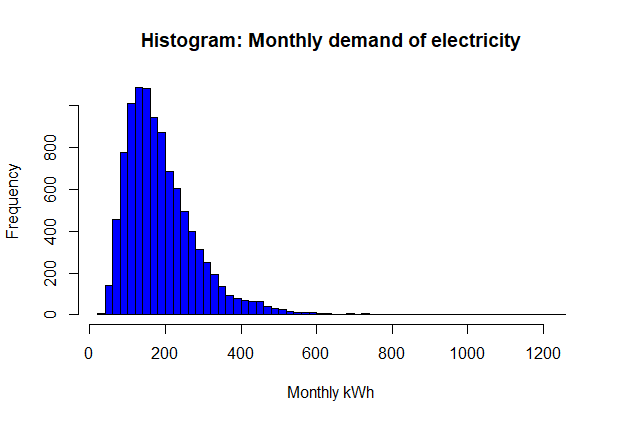
\includegraphics[width=340pt, height=200pt]{Chapters/chapter4/figures/PredDemElect.png}
	%%\centerline{\epsfig{/Chapters/chapter1/figures/cat.eps,width=.8\textheight,height=.4\textwidth}}
	\caption[List of figure caption goes here]{Histogram using the posterior predictive distribution of electricity demand}\label{fig41}
\end{figure}

 
\section{Multivariate linear regression: The conjugate normal-normal/inverse Wishart model}\label{sec44}

Let's study the multivariate regression setting where there are $N$-dimensional vectors ${\bf{y}}_m$, $m=1,2,\dots,M$ such that ${\bf{y}}_m={\bf{X}}\bm{\beta}_m+\mu_m$, ${\bf{X}}$ is the set of common regressors, and $\mu_m$ is the $N$-dimensional vector of stochastic errors for each equation such that ${\bf{U}}=[\mu_1 \ \mu_2 \ \dots \ \mu_M]\sim MN_{N,M}({\bf{0}}, {\bf{I}}_N, {\bm{\Sigma}})$, that is, a matrix variate normal distribution where $\bm{\Sigma}$ is the covariance matrix of each $i$-th row of ${\bf{U}}$, $i=1,2,\dots,N$, and we are assuming independence between the rows. Then, $vec({\bf U})\sim N_{N\times M}({\bf 0}, \bf{\Sigma}\otimes {\bf{I}}_N)$.\footnote{$vec$ denotes the vectorization operation, and $\otimes$ denotes the kronecker product.}

This framework can be written in matrix form

\begin{align*}
	\underbrace{
		\begin{bmatrix}
			y_{11} & y_{12} & \dots & y_{1M}\\
			y_{21} & y_{22} & \dots & y_{2M}\\
			\vdots & \vdots & \dots & \vdots\\
			y_{N1} & y_{N2} & \dots & y_{NM}\\
	\end{bmatrix}}_{\bf{Y}}
	&=
	\underbrace{\begin{bmatrix}
			x_{11} & x_{12} & \dots & x_{1K}\\
			x_{21} & x_{22} & \dots & x_{2K}\\
			\vdots & \vdots & \dots & \vdots\\
			x_{N1} & x_{N2} & \dots & x_{NK}\\
	\end{bmatrix}}_{\bf{X}}
	\underbrace{
		\begin{bmatrix}
			\beta_{11} & \beta_{12} & \dots & \beta_{1M}\\
			\beta_{21} & \beta_{22} & \dots & \beta_{2M}\\
			\vdots & \vdots & \dots & \vdots\\
			\beta_{K1} & \beta_{K2} & \dots & \beta_{KM}\\
	\end{bmatrix}}_{\bf{B}}\\
	&+
	\underbrace{\begin{bmatrix}
			\mu_{11} & \mu_{12} & \dots & \mu_{1M}\\
			\mu_{21} & \mu_{22} & \dots & \mu_{2M}\\
			\vdots & \vdots & \dots & \vdots\\
			\mu_{N1} & \mu_{N2} & \dots & \mu_{NM}\\
	\end{bmatrix}}_{\bf{U}}.
\end{align*}

Therefore, ${\bf{Y}}\sim N_{N\times M}({\bf{X}}{\bf{B}},\bf{\Sigma}\otimes {\bf{I}}_N)$,\footnote{We can write down the former expression in a more familiar way using vectorization properties,
$\underbrace{vec(Y)}_{\bf{y}}=\underbrace{({\bf{I}}_M\otimes {\bf{X}})}_{{\bf{Z}}}\underbrace{vec({\bf{B}})}_{\bm{\beta}}+\underbrace{vec({\bf{U}})}_{\mu}$, where ${\bf{y}}\sim N_{N\times M}({\bf{Z}}\bm{\beta},\bf{\Sigma}\otimes {\bf{I}}_N)$.}

\begin{align*}
	p({\bf{Y}}| {\bf{B}},{\bm{\Sigma}}, {\bf{X}})&\propto |{{\bf \Sigma}}|^{-N/2}\exp\left\lbrace -\frac{1}{2}tr\left[({\bf{Y}}-{\bf{X}}{\bf{B}})^{\top}({\bf{Y}}-{\bf{X}}{\bf{B}}){{\bf \Sigma}}^{-1}\right]\right\rbrace
	\\
	&=|{{\bf \Sigma}}|^{-N/2}\exp\left\lbrace -\frac{1}{2}tr\left[\left({\bf{S}}+({\bf{B}}-\widehat{\bf{B}})^{\top}{\bf{X}}^{\top}{\bf{X}}({\bf{B}}-\widehat{\bf{B}})\right){{\bf \Sigma}}^{-1}\right]\right\rbrace,
\end{align*}

where ${\bf{S}}= ({\bf{Y}}-{\bf{X}}\widehat{\bf{B}})^{\top}({\bf{Y}}-{\bf{X}}\widehat{\bf{B}})$, $\widehat{\bf{B}}= ({\bf{X}}^{\top}{\bf{X}})^{-1}{\bf{X}}^{\top}{\bf{Y}}$ (see Exercise 9).

The conjugate prior for this models is $\pi({\bf{B}},{\bf{\Sigma}})=\pi({\bf{B}}|{\bf{\Sigma}})\pi({\bf{\Sigma}})$ where $\pi({\bf{B}}|{\bf \Sigma})\sim N_{K\times M}({\bf{B}}_{0},{\bf{V}}_{0},{\bm{\Sigma}})$ and $\pi({\bm{\Sigma}})\sim IW({\bf{\Psi}}_{0},\alpha_{0})$, that is,

\begin{align*}
	\pi ({\bf{B}},{\bm{\Sigma}})\propto &\left|{\bm{\Sigma}} \right|^{-K/2}\exp\left\lbrace -\frac{1}{2}tr\left[({\bf{B}}-{\bf{B}}_{0})^{\top}{\bf{V}}_{0}^{-1}({\bf{B}}-{\bf{B}}_{0}){\bf \Sigma}^{-1}\right]\right\rbrace \\
	& \times \left|{\bf \Sigma} \right|^{-(\alpha_{0}+M+1)/2}\exp\left\lbrace -\frac{1}{2}tr \left[ {\bf{\Psi}}_{0} {\bf \Sigma}^{-1}\right] \right\rbrace.
\end{align*}

The posterior distribution is given by

\begin{align*}
	\pi({\bf{B}},{\bm{\Sigma}}|{\bf{Y}},{\bf{X}})&\propto  p({\bf{Y}}|{\bf{B}},{\bm{\Sigma}},{\bf{X}}) \pi({\bf{B}}| {\bf \Sigma})\pi({\bm{\Sigma}})\\
	&\propto \left|{\bm{\Sigma}} \right|^{-\frac{N+K+\alpha_{0}+M+1}{2}}\\
	&\times\exp\left\lbrace -\frac{1}{2}tr\left[(\bf{\Psi}_{0}+{\bf{S}} +({\bf{B}}-{\bf{B}}_{0})^{\top}{\bf{V}}_{0}^{-1}({\bf{B}}-{\bf{B}}_{0})\right.\right.\\
	&\left.\left.   +({\bf{B}}-\widehat{\bf{B}})^{\top}{\bf{X}}^{\top}{\bf{X}}({\bf{B}}-\widehat{\bf{B}}))\bf{\Sigma}^{-1}\right]\right\rbrace .
\end{align*}
Completing the squares on ${\bf{B}}$ and collecting the remaining terms in the bracket yields
{\footnotesize{
\begin{align*}
	{\bf{\Psi}}_{0}+{\bf{S}} +({\bf{B}}-{\bf{B}}_{0})^{\top}{\bf{V}}_{0}^{-1}({\bf{B}}-{\bf{B}}_{0})+({\bf{B}}-\widehat{\bf{B}})^{\top}{\bf{X}}^{\top}{\bf{X}}({\bf{B}}-\widehat{\bf{B}})
	& = ({\bf{B}}-{\bf{B}}_n)^{\top}{\bf{V}}_n^{-1}({\bf{B}}-{\bf{B}}_n)+{\bf{\Psi}}_n,
\end{align*}
}}
where 
\begin{align*}
	{\bf{B}}_n = &({\bf{V}}_{0}^{-1}+{\bf{X}}^{\top}{\bf{X}})^{-1}({\bf{V}}_{0}^{-1}{\bf{B}}_{0}+{\bf{X}}^{\top}{\bf{Y}})=({\bf{V}}_{0}^{-1}+{\bf{X}}^{\top}{\bf{X}})^{-1}({\bf{V}}_{0}^{-1}{\bf{B}}_{0}+{\bf{X}}^{\top}{\bf{X}}\widehat{\bf{B}}),\\
	{\bf{V}}_n = &({\bf{V}}_{0}^{-1}+{\bf{X}}^{\top}{\bf{X}})^{-1},\\
	{\bf{\Psi}}_n= &{\bf{\Psi}}_{0}+{\bf{S}}+{\bf{B}}_{0}^{\top}{\bf{V}}_{0}^{-1}{\bf{B}}_{0}+\widehat{\bf{B}}^{\top}{\bf{X}}^{\top}{\bf{X}}\widehat{\bf{B}}-{\bf{B}}_n^{\top}{\bf{V}}_n^{-1}{\bf{B}}_n.
\end{align*}
Thus, the posterior distribution can be written as
\begin{align*}
	\pi({\bf{B}},{\bf \Sigma}| {\bf{Y}}, {\bf{X}})\propto &\left|{\bf \Sigma} \right|^{-K/2}\exp\left\lbrace -\frac{1}{2} tr\left[({\bf{B}}-{\bf{B}}_n)^{\top}{\bf{V}}_n^{-1}({\bf{B}}-{\bf{B}}_n)   {\bf \Sigma}^{-1}\right]\right\rbrace \\
	\times & \left|{\bf \Sigma} \right|^{-\frac{N+\alpha_{0}+M+1}{2}}\exp\left\lbrace -\frac{1}{2} tr \left[ {\bf{\Psi}}_n{\bf \Sigma}^{-1}\right] \right\rbrace .
\end{align*}
That is $\pi({\bf{B}},{\bf \Sigma}| {\bf{Y}}, {\bf{X}})=\pi ({\bf{B}}| {\bf \Sigma},{\bf{Y}},{\bf{X}})\pi({\bf \Sigma}| {\bf{Y}},{\bf{X}})$ where $\pi({\bf{B}}| {\bf \Sigma},{\bf{Y}}, {\bf{X}}) \sim N_{K\times M}({\bf{B}}_n,{\bf{V}}_n,{\bf \Sigma})$ and $\pi({\bf \Sigma}| {\bf{Y}},{\bf{X}}) \sim IW({\bf{\Psi}}_n,{\alpha}_n)$, $\alpha_n= N+\alpha_{0}$. Observe again that we can write down the posterior mean as a weighted average between prior and sample information such that ${\bf{V}}_0\rightarrow\infty$ implies ${\bf{B}}_n\rightarrow\hat{{\bf{B}}}$, as we show in the univariate linear model.

The marginal posterior for ${\bf{B}}$ is given by
\begin{align*}
	\pi({\bf{B}}|{\bf{Y}},{\bf{X}})&\propto \int_{\bf{\mathcal{S}}} \left|{\bf \Sigma} \right|^{-(\alpha_n+K+M+1)/2}\\
	&\times\exp\left\lbrace -\frac{1}{2} tr\left\{\left[({\bf{B}}-{\bf{B}}_n)^{\top}{\bf{V}}_n^{-1}({\bf{B}}-{\bf{B}}_n)+{\bf{\Psi}}_n \right]  {\bf \Sigma}^{-1}\right\}\right\rbrace d{\bf{\Sigma}} \\
 	&\propto|({\bf{B}}-{\bf{B}}_n)^{\top}{\bf{V}}_n^{-1}({\bf{B}}-{\bf{B}}_n)+{\bf{\Psi}}_n|^{-(K+\alpha_n)/2}\\
 	&=\left[|{\bf{\Psi}}_n|\times|{\bf{I}}_K+{\bf{V}}_n^{-1}({\bf{B}}-{\bf{B}}_n){\bf{\Psi}}_n^{-1}({\bf{B}}-{\bf{B}}_n)^{\top}|\right]^{-(\alpha_n+1-M+K+M-1)/2}\\
 	&\propto|{\bf{I}}_K+{\bf{V}}_n^{-1}({\bf{B}}-{\bf{B}}_n){\bf{\Psi}}_n^{-1}({\bf{B}}-{\bf{B}}_n)^{\top}|^{-(\alpha_n+1-M+K+M-1)/2}.
\end{align*}

The second line uses the inverse Wishart distribution, the third line the Sylverter's theorem, and the last line is the kernel of a matrix t distribution, that is, ${\bf{B}}|{\bf{Y}},{\bf{X}}\sim T_{K\times M}({\bf{B}}_n,{\bf{V}}_n,{\bf{\Psi}}_n)$ with $\alpha_n+1-M$ degrees of freedom. 

Observe that $vec({\bf{B}})$ has mean $vec({\bf{B}}_n)$ and variance $({\bf{V}}_n\otimes{\bf{\Psi}}_n)/(\alpha_n-M-1)$ based on its marginal distribution. On the other hand, the variance based on the conditional distribution is ${\bf{V}}_n\otimes{\bf{\Sigma}}$, where the mean of ${\bf{\Sigma}}$ is ${\bf{\Psi}}_n/(\alpha_n-M-1)$.   

The marginal likelihood is the following,

\begin{align*}
	p({\bf{Y}})&=\int_{\mathcal{B}}\int_{\mathcal{S}}\left\{ (2\pi)^{-NM/2} |{{\bf \Sigma}}|^{-N/2}\exp\left\lbrace -\frac{1}{2}tr\left[{\bf{S}}+({\bf{B}}-\widehat{\bf{B}})^{\top}{\bf{X}}^{\top}{\bf{X}}({\bf{B}}-\widehat{\bf{B}})\right]{{\bf \Sigma}}^{-1}\right\rbrace\right.\\
	&\times (2\pi)^{-KM/2}\left|{\bf V}_0 \right|^{-M/2} \left|{\bm{\Sigma}} \right|^{-K/2}\exp\left\lbrace -\frac{1}{2}tr\left[({\bf{B}}-{\bf{B}}_{0})^{\top}{\bf{V}}_{0}^{-1}({\bf{B}}-{\bf{B}}_{0}){\bf \Sigma}^{-1}\right]\right\rbrace \\
	&\left. \times \frac{|\Psi_0|^{\alpha_0/2}}{2^{\alpha_0M/2}\Gamma_M(\alpha_0/2)} \left|{\bf \Sigma} \right|^{-(\alpha_{0}+M+1)/2}\exp\left\lbrace -\frac{1}{2}tr \left[ {\bf{\Psi}}_{0} {\bf \Sigma}^{-1}\right] \right\rbrace \right\} d{\bm{\Sigma}} d{\bf B}\\
	&=(2\pi)^{-M(N+K)/2}\left|{\bf V}_0\right|^{-M/2}\frac{|\Psi_0|^{\alpha_0/2}}{2^{\alpha_0M/2}\Gamma_M(\alpha_0/2)}\\
	&\times\int_{\mathcal{B}}\int_{\mathcal{S}} \left\{ \left|{\bf \Sigma} \right|^{-(\alpha_{0}+N+K+M+1)/2}\right.\\
	&\left. \exp\left\lbrace -\frac{1}{2}tr\left[{\bf{S}}+({\bf{B}}-\widehat{\bf{B}})^{\top}{\bf{X}}^{\top}{\bf{X}}({\bf{B}}-\widehat{\bf{B}})+({\bf{B}}-{\bf{B}}_{0})^{\top}{\bf{V}}_{0}^{-1}({\bf{B}}-{\bf{B}}_{0})+{\bf{\Psi}}_0\right]{{\bf \Sigma}}^{-1}\right\rbrace\right\}d{\bm{\Sigma}} d{\bf B}\\
	&=(2\pi)^{-M(N+K)/2}\left|{\bf V}_0\right|^{-M/2}\frac{|\Psi_0|^{\alpha_0/2}}{2^{\alpha_0M/2}\Gamma_M(\alpha_0/2)}2^{M(\alpha_n+K)/2}\Gamma_M((\alpha_n+K)/2)\\
	&\times \int_{\mathcal{B}}\left|{\bf{S}}+({\bf{B}}-\widehat{\bf{B}})^{\top}{\bf{X}}^{\top}{\bf{X}}({\bf{B}}-\widehat{\bf{B}})+({\bf{B}}-{\bf{B}}_{0})^{\top}{\bf{V}}_{0}^{-1}({\bf{B}}-{\bf{B}}_{0})+{\bf{\Psi}}_0\right|^{-(\alpha_n+K)/2}d{\bf{B}}\\
	&=(2\pi)^{-M(N+K)/2}\left|{\bf V}_0\right|^{-M/2}\frac{|\Psi_0|^{\alpha_0/2}}{2^{\alpha_0M/2}\Gamma_M(\alpha_0/2)}2^{M(\alpha_n+K)/2}\Gamma_M((\alpha_n+K)/2)\\
	&\times \int_{\mathcal{B}}\left|({\bf{B}}-\widehat{\bf{B}}_n)^{\top}{\bf{V}}_n^{-1}({\bf{B}}-\widehat{\bf{B}}_n)+{\bf{\Psi}}_n\right|^{-(\alpha_n+K)/2}d{\bf{B}}\\ 
	&=(2\pi)^{-M(N+K)/2}\left|{\bf V}_0\right|^{-M/2}\frac{|\Psi_0|^{\alpha_0/2}}{2^{\alpha_0M/2}\Gamma_M(\alpha_0/2)}2^{M(\alpha_n+K)/2}\Gamma_M((\alpha_n+K)/2)\\
	&\times \int_{\mathcal{B}}\left[|{\bf{\Psi}}_n|\times |{\bf{I}}_{K}+{\bf{V}}_n^{-1}({\bf{B}}-\widehat{\bf{B}}_n){\bf{\Psi}}_n^{-1}({\bf{B}}-\widehat{\bf{B}}_n)^{\top}|\right]^{-(\alpha_n+K)/2}d{\bf{B}}\\
	&=|{\bf{\Psi}}_n|^{-(\alpha_n+K)/2}(2\pi)^{-M(N+K)/2}\left|{\bf V}_0\right|^{-M/2}\frac{|\Psi_0|^{\alpha_0/2}2^{M(\alpha_n+K)/2}\Gamma_M((\alpha_n+K)/2)}{2^{\alpha_0M/2}\Gamma_M(\alpha_0/2)}\\
	&\times \int_{\mathcal{{\bf{B}}}}\left| {\bf{I}}_{K}+{\bf{V}}_n^{-1}({\bf{B}}-\widehat{\bf{B}}_n){\bf{\Psi}}_n^{-1}({\bf{B}}-\widehat{\bf{B}}_n)^{\top}\right|^{-(\alpha_n+1-M+K+M-1)/2}d{\bf{B}}\\
	&=|{\bf{\Psi}}_n|^{-(\alpha_n+K)/2}(2\pi)^{-M(N+K)/2}\left|{\bf V}_0\right|^{-M/2}\frac{|\Psi_0|^{\alpha_0/2}2^{M(\alpha_n+K)/2}\Gamma_M((\alpha_n+K)/2)}{2^{\alpha_0M/2}\Gamma_M(\alpha_0/2)}\\
	&\times \pi^{MK/2}\frac{\Gamma_M((\alpha_n+1-M+M-1)/2)}{\Gamma_M((\alpha_n+1-M+K+M-1)/2)}|{\bf{\Psi}}_n|^{K/2}|{\bf{V}}_n|^{M/2}\\
	&=\frac{|{\bf{V}}_n|^{M/2}}{|{\bf{V}}_0|^{M/2}}\frac{|{\bf{\Psi}}_0|^{\alpha_0/2}}{|{\bf{\Psi}}_n|^{\alpha_n/2}}\frac{\Gamma_M(\alpha_n/2)}{\Gamma_M(\alpha_0/2)}\pi^{-MN/2}.  
\end{align*}

The third equality follows from having the kernel of a inverse Wishart distribution, the fifth from the Silvester's theorem, and the seventh from having the kernel of a matrix t distribution.

Observe that this last expression is the multivariate case of the marginal likelihood of the univariate regression model. Taking into account that 
\begin{align*}
	({\bf{A}}+{\bf{B}})^{-1}&={\bf{A}}^{-1}-({\bf{A}}^{-1}+{\bf{B}}^{-1})^{-1}{\bf{A}}^{-1}\\
	&={\bf{B}}^{-1}-({\bf{A}}^{-1}+{\bf{B}}^{-1})^{-1}{\bf{B}}^{-1}\\
	&={\bf{A}}^{-1}({\bf{A}}^{-1}+{\bf{B}}^{-1}){\bf{B}}^{-1},
\end{align*} 

we can show that ${\bf{\Psi}}_{n}={\bf{\Psi}}_{0}+{\bf{S}}+(\hat{\bf{B}}-{\bf{B}}_{0})^{\top}{\bf{V}}_{n}(\hat{\bf{B}}-{\bf{B}}_{0})$ (see Exercise 7). Therefore, the marginal likelihood rewards fit (smaller sum of squares, ${\bf{S}}$), similarity between prior and sample information regarding location parameters, and information gains in variability from ${\bf{V}}_0$ to ${\bf{V}}_n$.   

Given a matrix of regressors ${\bf{X}}_0$ for $N_0$ unobserved units, the predictive density of ${\bf{Y}}_0$ given ${\bf{Y}}$, $\pi({\bf{Y}}_0|{\bf{Y}})$ is a matrix t distribution $T_{N_0,M}(\alpha_n-M+1,{\bf{X}}_0{\bf{B}}_n,{\bf{I}}_{N_0}+{\bf{X}}_0{\bf{V}}_n{\bf{X}}_0^{\top},{\bf{\Psi}}_n)$ (see Exercise 6). Observe that the prediction is centered at ${\bf{X}}_0{\bf{B}}_n$, and the covariance matrix of $vec({\bf{Y}}_0)$ is $\frac{({\bf{I}}_{N_0}+{\bf{X}}_0{\bf{V}}_n{\bf{X}}_0^{\top})\otimes{\bf{\Psi}}_n}{\alpha_n-M-1}$.  

\section{Summary}\label{sec45}
We introduce the conjugate family models for discrete and continuous data. These models are the basic Bayesian framework to due its mathematical tractability as we get closed-form expressions for the posterior distributions, the marginal likelihood, and the predictive distribution. We also present the Bayesian linear univariate and multivariate regression frameworks under conjugate families. This is the cornerstone to perform regression analysis in the Bayesian setting. 

\section{Exercises}\label{sec46}

\begin{enumerate}
	\item Write in the canonical form the distribution of the Bernoulli example, and find the mean and variance of the sufficient statistic.
	
	\item Given a random sample $\mathbf{y}=[y_1,y_2,\dots,y_N]^{\top}$ from $N$ \textit{binomial experiments} each having known size $n_i$ and same unknown probability $\theta$. Show that $p(\mathbf{y}|\theta)$ is in the exponential family, and find the posterior distribution, the marginal likelihood and the predictive distribution of the binomial-beta model assuming the number of trials is known.
	
	\item Given a random sample $\mathbf{y}=[y_1,y_2,\dots,y_N]^{\top}$ from a \textit{exponential distribution}. Show that $p(\mathbf{y}|\lambda)$ is in the exponential family, and find the posterior distribution, marginal likelihood and predictive distribution of the exponential-gamma model.
	
	\item Given $\mathbf{y}\sim N_N(\bm{\mu},\bm{\Sigma})$, that is, a \textit{multivariate normal distribution} show that $p(\mathbf{y}|\bm{\mu},\bm{\Sigma})$ is in the exponential family.
	
	\item Find the marginal likelihood in the normal/inverse-Wishart model.
	
	\item Find the posterior predictive distribution in the normal/inverse-Wishart model, and show that ${\bf{Y}}_0|{\bf{Y}}\sim T_{N_0,M}(\alpha_n-M+1,{\bf{X}}_0{\bf{B}}_n,{\bf{I}}_{N_0}+{\bf{X}}_0{\bf{V}}_n{\bf{X}}_0^{\top},{\bf{\Psi}}_n)$.
	
	\item Show that $\delta_n=\delta_0+({\bf{y}}-{\bf{X}}\hat{\bm{\beta}})^{\top}({\bf{y}}-{\bf{X}}\hat{\bm{\beta}})+(\hat{\bm{\beta}}-\bm{\beta}_0)^{\top}(({\bf{X}}^{\top}{\bf{X}})^{-1}+{\bf{B}}_0)^{-1}(\hat{\bm{\beta}}-\bm{\beta}_0)$ in the linear regression model, and that ${\bf{\Psi}}_{n}={\bf{\Psi}}_{0}+{\bf{S}}+(\hat{\bf{B}}-{\bf{B}}_{0})^{\top}{\bf{V}}_{n}(\hat{\bf{B}}-{\bf{B}}_{0})$ in the linear multivariate regression model. 
			
	\item Show that in the linear regression model $\bm{\beta}_n^{\top}({\bf{B}}_n^{-1}-{\bf{B}}_n^{-1}{\bf{M}}^{-1}{\bf{B}}_n^{-1})\bm{\beta}_n={\bf{\bm{\beta}}}_{**}^{\top}{\bf{C}}{\bf{\bm{\beta}}}_{**}$ and $\bm{\beta}_{**}={\mathbf{X}}_0\bm{\beta}_n$.
	
	\item Show that $({\bf{Y}}-{\bf{X}}{\bf{B}})^{\top}({\bf{Y}}-{\bf{X}}{\bf{B}})={\bf{S}}+({\bf{B}}-\widehat{\bf{B}})^{\top}{\bf{X}}^{\top}{\bf{X}}({\bf{B}}-\widehat{\bf{B}})$ where ${\bf{S}}= ({\bf{Y}}-{\bf{X}}\widehat{\bf{B}})^{\top}({\bf{Y}}-{\bf{X}}\widehat{\bf{B}})$, $\widehat{\bf{B}}= ({\bf{X}}^{\top}{\bf{X}})^{-1}{\bf{X}}^{\top}{\bf{Y}}$ in the multivariate regression model.
	
	\item \textbf{What is the probability that the Sun will rise tomorrow?}
	
	This is the most famous Richard Price's example developed in the Appendix of the Bayes' theorem paper \cite{bayes1763lii}. Here, we implicitly use \textit{Laplace's Rule of Succession} to solve this question. In particular, if we were a priori uncertain about the probability the Sun will rise on a specified day, we can assume a prior uniform distribution over (0,1), that is, a beta (1,1) distribution. Then, what is the probability that the Sun will rise?
	
	
	\item Using information from Public Policy Polling in September 27th-28th for the 2016 presidential five-way race in USA, there are 411, 373 and 149 sampled people supporting Hillary Clinton, Donald Trump and other, respectively. 
	
	\begin{itemize}
		\item Find the posterior probability of the percentage difference of people supporting Hillary versus Trump according to this data using a non-informative prior, that is, $\alpha_0=[1 \ 1 \ 1]$ in the multinomial-Dirichlet model. What is the probability of having more supports of Hillary vs Trump?
		
		\item What is the probability that sampling one hundred independent individuals 44, 40 and 16 support Hillary, Trump and other, respectively?  
	\end{itemize}

\item \textbf{Math test example continues}

You have a random sample of math scores of size $N=50$ from a normal distribution, $Y_i\sim \mathcal{N}(\mu, \sigma)$. The sample mean and variance are equal to $102$ and $10$, respectively. Using the normal-normal/inverse-gamma model where $\mu_0=100$, $\beta_0=1$, $\alpha_0=\delta_0=0.001$

\begin{itemize}
	\item Get a 95\% confidence and credible interval for $\mu$.
	\item What is the posterior probability that $\mu > 103$?  
\end{itemize} 

%\item In the optimal tangency portfolio example, what are the equations for $\mu_{T+\kappa}=\mu_n$ and ${\bm{\Sigma}}_{T+\kappa}$? Use these equations to find the optimal weights six periods ahead using the tech stocks. 

\item \textbf{Demand of electricity example continues}

Set $c_0$ such that maximizes the marginal likelihood in the specifications with and without electricity price in the example of demand of electricity (empirical Bayes). Then, calculate the Bayes factor, and conclude if there is evidence supporting the inclusion of the price of electricity in the demand equation.

\item \textbf{Utility demand}

Use the file \textit{Utilities.csv} to estimate a multivariate linear regression model where $\mathbf{Y}_i=\left[\log(\text{electricity}_i) \ \log(\text{water}_i) \ \log(\text{gas}_i)\right]$ as function of $\log(\text{electricity price}_i)$, $\log(\text{water price}_i)$, $\log(\text{gas price}_i)$, $\text{IndSocio1}_i$, $\text{IndSocio2}_i$, $\text{Altitude}_i$, $\text{Nrooms}_i$, $\text{HouseholdMem}_i$, $\text{Children}_i$, and $\log(\text{Income}_i)$, where electricity, water and gas are monthly consumption of electricity (kWh), water (m$^3$) and gas (m$^3$), and other definitions are given in the Example of Section \ref{sec43}. Omit households that do not consume any of the utilities in this exercise.  

Set a non-informative prior framework, $\mathbf{B}_0=\left[0\right]_{11\times 3}$, $\mathbf{V}_0=1000 \mathbf{I}_{11}$, $\mathbf{\Psi}_0=1000 \mathbf{I}_{3}$ and $\alpha_0=3$, where we have $K=11$ (regressors plus intercept) and $M=3$ (equations) in this exercise.

\begin{enumerate}
	\item Find the posterior mean estimates and the highest posterior density intervals at 95\% of $\mathbf{B}$ and $\bm{\Sigma}$. Use the marginal distribution and the conditional distribution to obtain the posterior estimates of  $\mathbf{B}$, and compare the results.
	\item Find the Bayes factor comparing the baseline model in this exercise with the same specification but using the income in dollars. Now, calculate the Bayes factor using the income in thousand dollars. Is there any difference?
	\item Find the predictive distribution for the monthly demand of electricity, water and gas in the baseline specification of a household located in the lowest socioeconomic condition in a municipality located below 1000 meters above the sea level, 2 rooms, 3 members with children, a monthly income equal to USD 500, an electricity price equal to USD/kWh 0.15, a water price equal to USD/M$^3$ 0.70, and a gas price equal to USD/M$^3$ 0.75. 
\end{enumerate} 
	

\end{enumerate}



